\documentclass[12pt,a4paper,twoside]{report}

% link to wordpage source \href{https://campuscvut-my.sharepoint.com/:w:/g/personal/hasplvoj_cvut_cz/EY8pybo8CfdNmaBXNMXVtx0BKKOaEe7kFf99Fhh3AoGY8Q?e=3V3gST}{\color{blue}{wordpage}}

\usepackage{packages/cvut}
% Graphics
\usepackage[colorlinks=true,linkcolor=black,anchorcolor=black,citecolor=black,filecolor=black,menucolor=black,runcolor=black,urlcolor=black]{hyperref}
\usepackage[labelsep=period]{caption}
%\usepackage{subcaption}
\usepackage{graphicx}
\usepackage{pdfpages}
\usepackage{subfig}
\usepackage{float}

% Math
\usepackage{amsthm}
\usepackage{amsmath}
\usepackage{amsfonts}

% Lists
\usepackage{enumerate}
\usepackage{paralist}
\usepackage{acronym}
\usepackage[nonumberlist]{glossaries} % troubleshooting

% Tables
\usepackage{booktabs}
\usepackage{multirow}
\usepackage{multicol}
\usepackage{tabularx}
\usepackage{etoolbox}

% Algorithms
\usepackage{algorithm}
\usepackage{algpseudocode}

% Title etc.
\usepackage{chngcntr}
\usepackage{cite}
\usepackage{titlesec}

% etc.
\usepackage{setspace}
\usepackage{color}
\usepackage{pdflscape}
\usepackage{afterpage}
\usepackage[nottoc]{tocbibind} 
\usepackage[toc]{appendix}
\usepackage{listings}
%\usepackage[resetlabels,labeled]{multibib}
%\usepackage[T1]{fontenc}
%\usepackage{chngcntr}
%\counterwithin{Figure}{chapter}


% TODO pridat article jako zdroj globaldata do INTRA

\setlength{\parindent}{0pt}                 % creates normal paragrapsh separation
\setlength{\parskip}{10pt}                  % creates normal paragraph separation

\graphicspath{ {./images/} }                % where to look for images in \includegraphics{xxx.png} command

\setacronymstyle{long-sc-short}
% \usepackage{subfigure}
 \setacronymstyle{long-short}

%\counterwithout{figure}{chapter}
%\counterwithout{equation}{section} % undo numbering system provided by phstyle.cls
%\counterwithout{equation}{chapter} % implement desired numbering system

 \newtheorem{my_theorem}{Theorem} 
 \newtheorem{Assumption}{\bf AS}
 \newtheorem{my_lemma}{Lemma}
 \newtheorem{my_prep}{Proposition}
 \newtheorem{my_remark}{Remark}
 \newtheorem{my_corr}{Corollary}
 
 \DeclareMathOperator*{\argmin}{\arg\!\min}
 \DeclareMathOperator*{\argmax}{\arg\!\max}
 
 
 \definecolor{GreenTable}{cmyk}{0.59,0,0.88,0.27}
 
 	\providecommand{\keywords}[1]{\vspace{4pt}\textbf{\textit{Keywords: }} #1}
 	\providecommand{\keywordscz}[1]{\vspace{4pt}\textbf{\textit{Klíčová slova: }} #1}
 	
\pdfminorversion=7
\makeatletter
\def\bstctlcite{\@ifnextchar[{\@bstctlcite}{\@bstctlcite[@auxout]}}
\def\@bstctlcite[#1]#2{\@bsphack
	
	\@for\@citeb:=#2\do{%
		\edef\@citeb{\expandafter\@firstofone\@citeb}%
		\if@filesw\immediate\write\csname
		#1\endcsname{\string\citation{\@citeb}}\fi}%
	\@esphack}
\makeatother

\DeclareRobustCommand{\ttfamily}{\fontencoding{T1}\fontfamily{lmtt}\selectfont}

%\usepackage{titlesec}
% defines things like author and date or field of study for titlepage
\DeclareMathOperator*{\argmaxA}{arg\,max}
\DeclareMathOperator*{\argminA}{arg\,min} 
\title {Development of Testbed for Vehicular Edge Computing}
\author{Vojtěch Hašpl}


\date{My 2023}

\argument{supervisor}{Ing. Jan Plachý, Ph.D.}
\argument{cosupervisor}{}
\argument{department}{Department of Telecommunication Engineering}
\argument{programme}{Electronics and Communications}
\argument{specialization}{-}
\argument{dateyear}{2023}
\argument{datemonth}{May}
\argument{location}{Prague}
\argument{fulldate}{May,~2023}
\argument{fulldatecz}{25. května~2023}
 \renewcommand{\chaptername}{}

%\addto\captionsczech{\renewcommand{\keywordsname}{Klíčová slova}} 
 \makeatletter
 	
% \def\@makechapterhead#1{%
% \vspace*{20\p@}%
% {\parindent \z@ \raggedright \normalfont
% %\ifnum \c@secnumdepth >\m@ne
% % \huge\bfseries \@chapapp\space \thechapter
% % \par\nobreak
% % \vskip 20\p@
% %\fi
% \interlinepenalty\@M
% \Huge \bfseries \thechapter. \Huge \bfseries #1\par\nobreak
% \vskip 40\p@
% }}
\titleformat{\chapter}{\huge\bfseries}{\thechapter.}{20pt}{\huge\bfseries}
 \makeatother
% \renewcommand{\bibname}{References}
 

 \newenvironment{spodnitext}[1]{
 	\cleardoublepage
 	\null
 	\vfill
 	\section*{#1}
 	}{
 	\vspace{10mm}
 	}
 	
 
% 	\renewcommand{\bibname}{References} 
 
 
 \AtBeginDocument{\renewcommand{\bibname}{References}}	
 \def\@makechapterhead#1{%
 	%%%%\vspace*{50\p@}% %%% removed!
 	{\parindent \z@ \raggedright \normalfont
 		\ifnum \c@secnumdepth >\m@ne
 		\huge\bfseries \@chapapp\space \thechapter
 		\par\nobreak
 		\vskip 20\p@
 		\fi
 		\interlinepenalty\@M
 		\Huge \bfseries #1\par\nobreak
 		\vskip 20\p@
 	}}
 	\def\@makeschapterhead#1{%
 		%%%%%\vspace*{50\p@}% %%% removed!
 		{\parindent \z@ \raggedright
 			\normalfont
 			\interlinepenalty\@M
 			\Huge \bfseries #1\par\nobreak
 			\vskip 1\p@
 		}}

\renewcommand*{\glsgroupskip}{}

% -----------------------
%  listings definitions
% -----------------------
\lstnewenvironment{flask}[1][]
{
    \lstset{
        language=Python,
        frame=single,
        basicstyle=\small\ttfamily,
        keywordstyle=\bfseries\color{blue},
        stringstyle=\color{red},
        commentstyle=\color{green},
        showstringspaces=false,
		tabsize=4,
        captionpos=b,
        numbers=left,
        numbersep=5pt,
        #1,
		breaklines,
		float
    }
}{}

% 	
\bibliographystyle{IEEEtran}
%\bibliography{IEEEabrv,minimum}
%\bibliographystyle{ieeetr}	
%\makenoidxglossaries

% ---------------------
%   Listing Acronyms
% ---------------------
\newacronym{iot}{IoT}{Internet of Things}
\newacronym{sdo}{SDO}{Standard Defining Organization}
\newacronym{3gpp}{3GPP}{Third Generation Partnership Project}
\newacronym{etsi}{ETSI}{Eurupean Telecommunication Standard Institution}
\newacronym{o-ran}{O-RAN}{Open Radio Access Network}
\newacronym{sms}{SMS}{Short Message Service}
\newacronym{vr}{VR}{Virtual Reality}
\newacronym{ran}{RAN}{Radio Access Network}
\newacronym{nr}{NR}{New Radio}
\newacronym{sba}{SBA}{Service Based Architecture}
\newacronym{ec}{EC}{Edge Computing}
\newacronym{cc}{CC}{Cloud Computing}
\newacronym{avs}{AVs}{Autonomous Vehicles}
\newacronym{mec}{MEC}{Multi-Access Edge Computing}
\newacronym{isg}{ISG}{Industry Specification Group}
\newacronym{vec}{VEC}{Vehicular Edge Computing}
\newacronym{b2b}{B2B}{Business-to-Business}
\newacronym{embb}{eMBB}{Enhanced Mobile Broadband}
\newacronym{mmtc}{mMTC}{Massive Machine Type Communication}
\newacronym{urllc}{URLLC}{Ultra Reliable Low Latency Communication}
\newacronym{nfv}{NFV}{Network Function Virtualization}
\newacronym{sdn}{SDN}{Software Defined Networking}
\newacronym{cups}{CUPS}{Control and User Plane Separation}
\newacronym{epc}{EPC}{Evolved Packet Core}
\newacronym{nfs}{NF}{Network Functions}
\newacronym{apis}{API}{Application Programmable Interface}
\newacronym{http}{HTTP}{Hypertext Transfer Protocol}
\newacronym{rest}{REST}{Representational State Transfer}
\newacronym{ue}{UE}{User Equipment}
\newacronym{upf}{UPF}{User Plane Function}
\newacronym{dn}{DN}{Data Network}
\newacronym{cn}{CN}{Core Network}
\newacronym{nssf}{NSSF}{Network Slice Selection Function}
\newacronym{nef}{NEF}{Network Exposure Funciton}
\newacronym{ausf}{AUSF}{Authentication Server Function}
\newacronym{nrf}{NRF}{Network Repository Function}
\newacronym{amf}{AMF}{Access and Mobility Management Function}
\newacronym{pcf}{PCF}{Policy Control Function}
\newacronym{smf}{SMF}{Session Management Function}
\newacronym{udm}{UDM}{Unified Data Management}
\newacronym{af}{AF}{Application Funciton}
\newacronym{pdu}{PDU}{Packet Data Unit}
\newacronym{qos}{QoS}{Quality of Service}
\newacronym{rrc}{RRC}{Radio Resource Control}
\newacronym{ul cl}{UL CL}{Uplink Classifier}
\newacronym{fes}{FEs}{Functional Entities}
\newacronym{mec apps}{MEC apps}{MEC Applications}
\newacronym{mp}{Mp}{MEC platform functionality reference point}
\newacronym{mm}{Mm}{MEC Management reference point}
\newacronym{mx}{Mx}{Reference point connecting to external entities}
\newacronym{oss}{OSS}{Operations Support System}
\newacronym{ualcmp}{UALCMP}{User Application Lifecycle Management Proxy}
\newacronym{meo}{MEO}{MEC Orchestrator}
\newacronym{mepm}{MEPM}{MEC Platform Manager}
\newacronym{vim}{VIM}{Virtualization Infrastructure Manager}
\newacronym{vm}{VM}{Virtual Machine}
\newacronym{k8s}{k8s}{Kubernetes}
\newacronym{cvb}{CVB}{Connected Vehicles Blueprint}
\newacronym{ealtedge}{EALTEdge}{Enterprise Application on Lightweight Telco Edge}
\newacronym{pcei}{PCEI}{Public Cloud Edge Interface}
\newacronym{openness}{OpenNESS}{Open Network Edge Services Software}
\newacronym{oai}{OAI}{OpenAirInterface}
\newacronym{osa}{OSA}{OpenAirInterface Software Alliance}
\newacronym{ll-mec}{LL-MEC}{Low-Latency MEC}
\newacronym{mep}{MEP}{MEC Platform}
\newacronym{rnis}{RNIS}{Radio Network Information Service}
\newacronym{enb}{eNB}{evolved NodeB}
\newacronym{gnb}{gNB}{new generation NodeB}
\newacronym{tcp}{TCP}{Transmission Control Protocol}
\newacronym{ip}{IP}{Internet Protocol}
\newacronym{sdap}{SDAP}{Service Data Application Protocol}
\newacronym{pdcp}{PDCP}{Packet Data Convergence Protocol}
\newacronym{rlc}{RLC}{Radio Link Control}
\newacronym{mac}{MAC}{Media Access Control}
\newacronym{phy}{PHY}{Physical Layer}
\newacronym{nas}{NAS}{Non-Access Stratum}
\newacronym{rtt}{RTT}{Rount Trip Time}
\newacronym{tdd}{TDD}{Time Division Duplex}
\newacronym{fdd}{FDD}{Frequency Division Duplex}
\newacronym{nfapi}{nFAPI}{Network Functional API}
\newacronym{cots}{COTS}{Customer Off-The-Shelf}
\newacronym{udr}{UDR}{Unified Data Repository}
\newacronym{flexric}{FlexRIC}{Flexible RAN Intelligent Controller}
\newacronym{flexcn}{FlexCN}{Flexible Core Controller}

\makeglossaries

% capton setup
%\captionsetup[figure]{name=Figure}

\setstretch{1.15}

% -----------------------
% THE BEGIN DOCUMENT HERE
% -----------------------
\begin{document}

% -----------------------
%        Titlepage
% -----------------------
\maketitle

% -----------------------
%      Assignment
% -----------------------
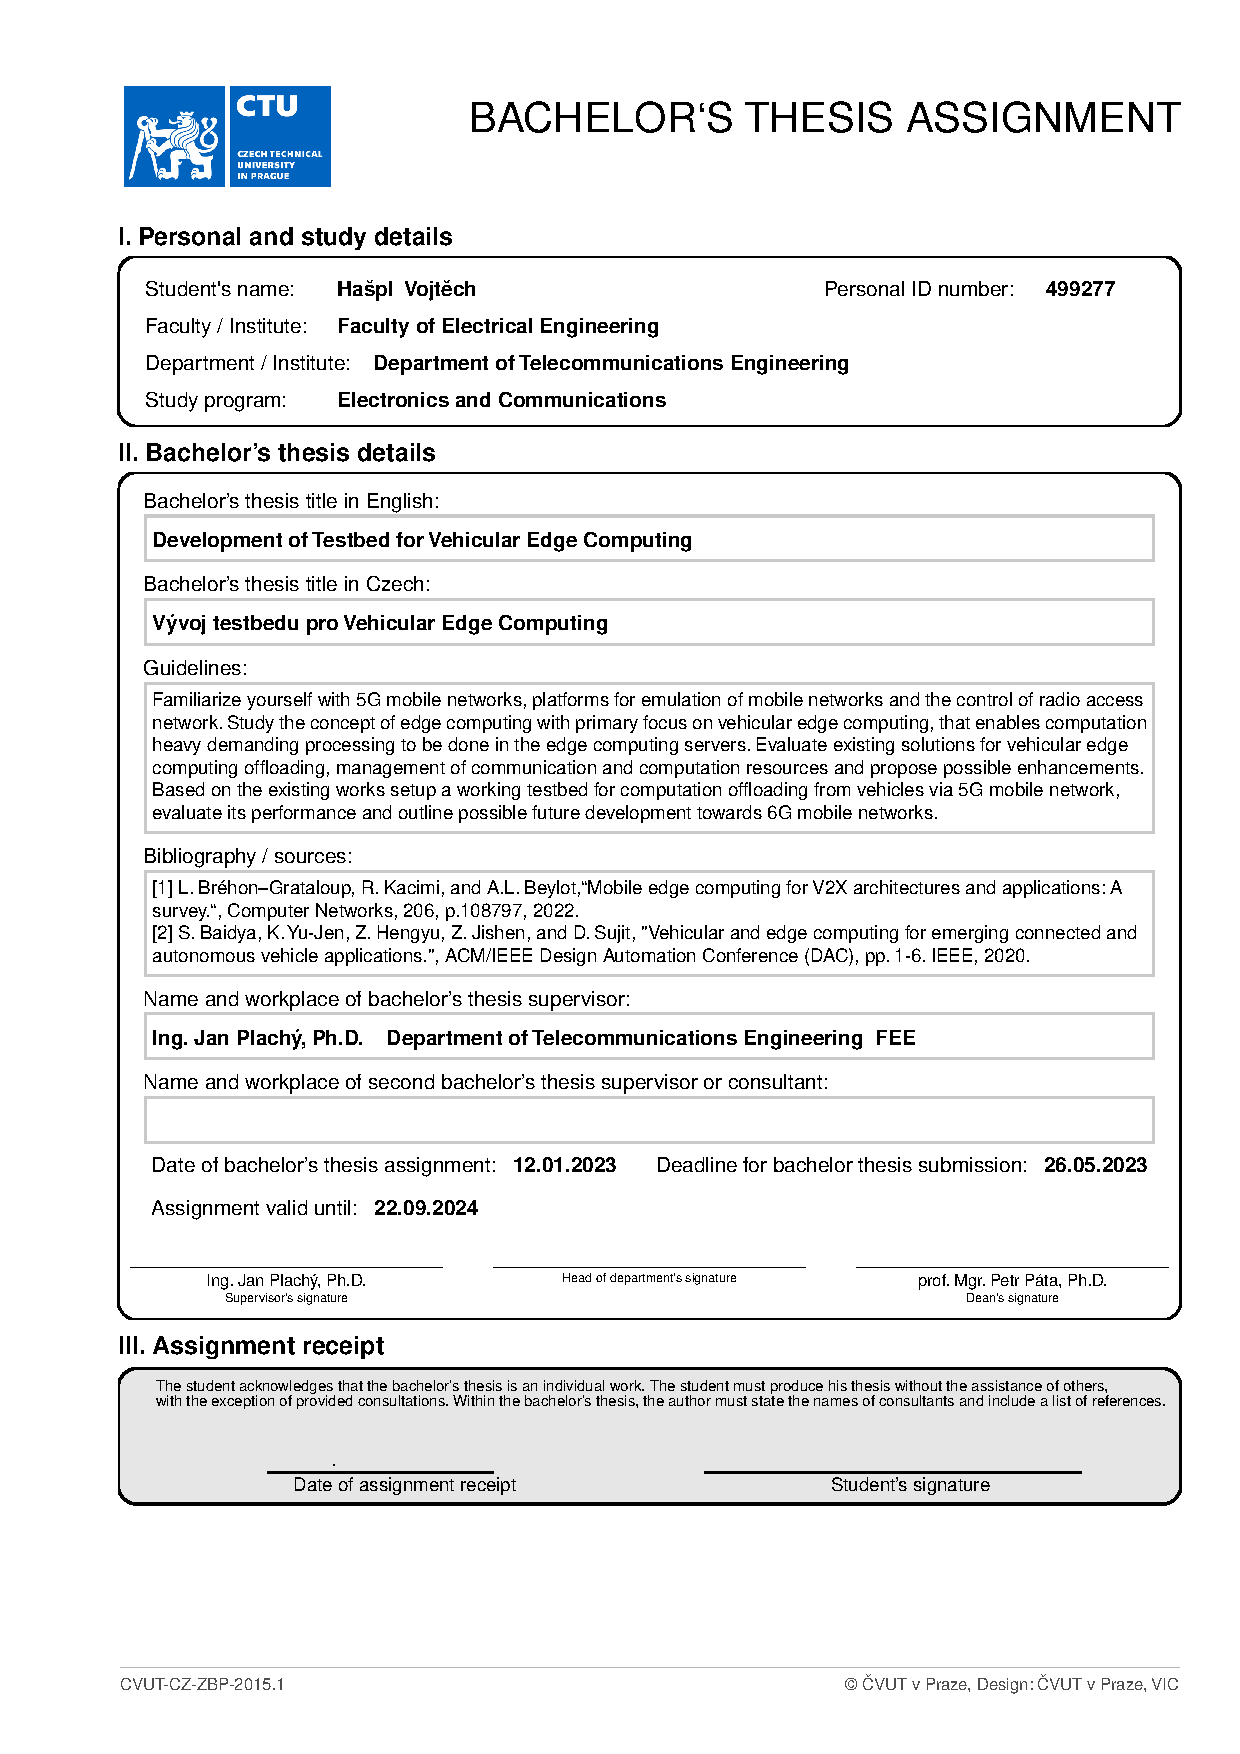
\includepdf{assignment/assignment_eng.pdf}


% -----------------------
%      Statement
% -----------------------
\makestatement


%\pagestyle{empty}
\pagenumbering{roman}


% -----------------------
%    Acknowledgement
% -----------------------
\chapter*{Acknowledgements}
	% \addcontentsline{toc}{chapter}{Acknowledgments}
	Thank you


% -----------------------
%        Abstracts
% -----------------------
\chapter*{Abstract}
	% \addcontentsline{toc}{chapter}{Abstract}	% comment to omit abstract from toc
	% ABSTRACT	
\keywords{mobile networks, multi-access edge computing, vehicular edge computing, task offloading, autonomous vehicles}
%
%fill in abstract
%
\newpage

\chapter*{Abstrakt}
	% \addcontentsline{toc}{chapter}{Abstrakt}	% comment to omit abstract from toc
\keywordscz{mobilní sítě, multi-access edge computing, vehicular edge computing, přesun výpočtů, autonomn\'i vozidla}
%
%fill in abstract
%
\newpage

% -----------------------
%        TOC
% -----------------------
\tableofcontents			

% -----------------------
%  GLOSSARIES (ABBREV)
% -----------------------
\glsaddallunused
\printglossary[type=\acronymtype,title={List of Abbreviations}]	% prints glossaries alphabetically

% -----------------------
%   List of Figures- WIP
% -----------------------


%\newpage
%\thispagestyle{empty}
%\mbox{}
\newpage

\setcounter{page}{1}
%\end{otherlanguage}
\pagenumbering{arabic}

\setstretch{1.15}
\chapter{Introduction}
Mobile networks are seen as a key enabler for emerging services and applications in internet of things (IoT) or vehicular sector, whose requirements on data rate and latency are ever increasing. This drives the need for innovation and development. The development of mobile networks follows standards defined by multiple standard defining organizations (SDO). Third Generation Partnership Project (3GPP) is a consortium of several regional institutions that define exact standards for all aspects of mobile networks such as architecture, protocols, interfaces, modulation techniques etc. The European SDO taking part in 3GPP is European Telecommunications Standard Institution (ETSI). 

The development of mobile networks started in 1980s with the first generation of mobile networks (1G) and focused on analog communication only and enabled voice calls \cite{sauter2017history}. The 1G was followed by 2G which switched from analog to digital communication and introduced short messages service (SMS) \cite{sauter2017history}. 3G mainly focused on enhancing data rates to enable multimedia applications such as video streaming \cite{sauter2017history}. 4G then disrupted mobile networks design by switching to fully IP based architecture and further enhancing data rates and decreasing latency \cite{sauter2017history,dahlman20134g}. 

The deployment of 5G started in 2019 and is still ongoing. Evolving from 4G, 5G was tasked with providing support for not only fast internet access, but also massive machine-type communication and mission critical communication \cite{dahlman20205g}. The goal of these requirements was to develop a flexible mobile network, capable of supporting novel applications such as virtual reality (VR), IoT or connected vehicles. The result is a redesigned 5G core network (CN) that serves as a flexible platform, capable of integrating novel applications and techniques like edge computing \cite{sabella-mec-sw-dev}. 

Edge computing (EC) can be described as an extension of cloud computing to the network edge \cite{sabella-mec-sw-dev}. Cloud computing (CC) is a computing paradigm that enables access to a pool of resources, e.g. (storage, computing, applications and services) via a network \cite{mell2011nistCC}. By bringing the resources closer to the user, to the network edge, EC can offer services with minimal latency, which is critical for applications such as autonomous vehicles (AVs). A specific standardized implementation of edge computing is called multi-access edge computing (MEC). MEC is an access agnostic EC model, which addresses user mobility through wireless access technologies. The leading international SDO regarding MEC is ETSI MEC, whose aim is to create an open standardized environment allowing for seamless integration of applications from vendors, service providers as well as third parties \cite{etsi-web}.  In this thesis, standards developed by ETSI MEC will be exploited. 

MEC would benefit various use cases such as IoT, augmented reality, location services or AVs \cite{etsi-web}. AVs require processing large amounts of data in order to recognize the surrounding environment and decide the best next action (slow down, speed up, turn etc.). This is a computationally demanding process, and the vehicles computation capacity is limited, compared to cloud. As shown in recent research \cite{zhao2019towards}, the computation required for level-4 and level-5 AVs requires server grade hardware. That is where MEC could be leveraged to offload some of the data processing to the network edge. This would drive down the vehicles’ cost and power consumption, while keeping the communication latency low. The utilization of MEC for vehicular applications is referred to as vehicular edge computing (VEC). 

As of today, VEC is still a work in progress. To provide a sufficient computation offloading from vehicles, algorithms for allocation of computation and communication resources need to be developed and evaluated. Therefore, this thesis focuses on developing a functional testbed for VEC. First, integration of MEC in 5G networks is explained. Then, in chapter 3, some existing open source platforms for emulating network edge are evaluated. Chapters 4 and 5 provide a more detailed description of the chosen platforms for emulation of edge and mobile network. Chapter 6 explains the integration of both platforms to form a functional testbed. Chapter 7 provides testbed evaluation and measurements. Finally, in last chapter, the thesis is concluded and future work outlined. 

TESTING References
\cite{ETSI:GS:MEC003,ETSI:WP:28,ETSI:WP:24}

\chapter{MEC \& 5G}
The aim of this chapter is to provide a detailed description of integration of MEC into 5G mobile networks. Although 5G is not a prerequisite for MEC deployment, with ETSI describing MEC and 4G integration in [h], 5G is the superior radio access technology for MEC. Contrary to 4G, 5G was designed to enable seamless integration of MEC [i] and works with lower latency [a], which is a crucial parameter for edge applications such as AVs.  In this chapter, both 5G  and MEC system architectures are described, before the final section of this chapter provides a framework for integration of MEC system into 5G CN.

\section{Key concepts in 5G}
The evolution from 4G to 5G has not focused only on providing improved experience for end users through enhancing communication data rates and decreasing latency. One of the main goals of 5G development has been to introduce industry businesses as new customers to mobile networks’ vendors [k]. To achieve that, two new industry oriented usage scenarios have been introduced to complement the end user oriented one – Enhanced Mobile Broadband (eMBB). The newly introduced usage scenarios are Massive Machine-Type Communication (mMTC) and Ultra-Reliable Low Latency Communication (URLLC) [k]. All three mentioned service grades are illustrated in Figure [1].
\begin{figure}[ht]
	\centering
	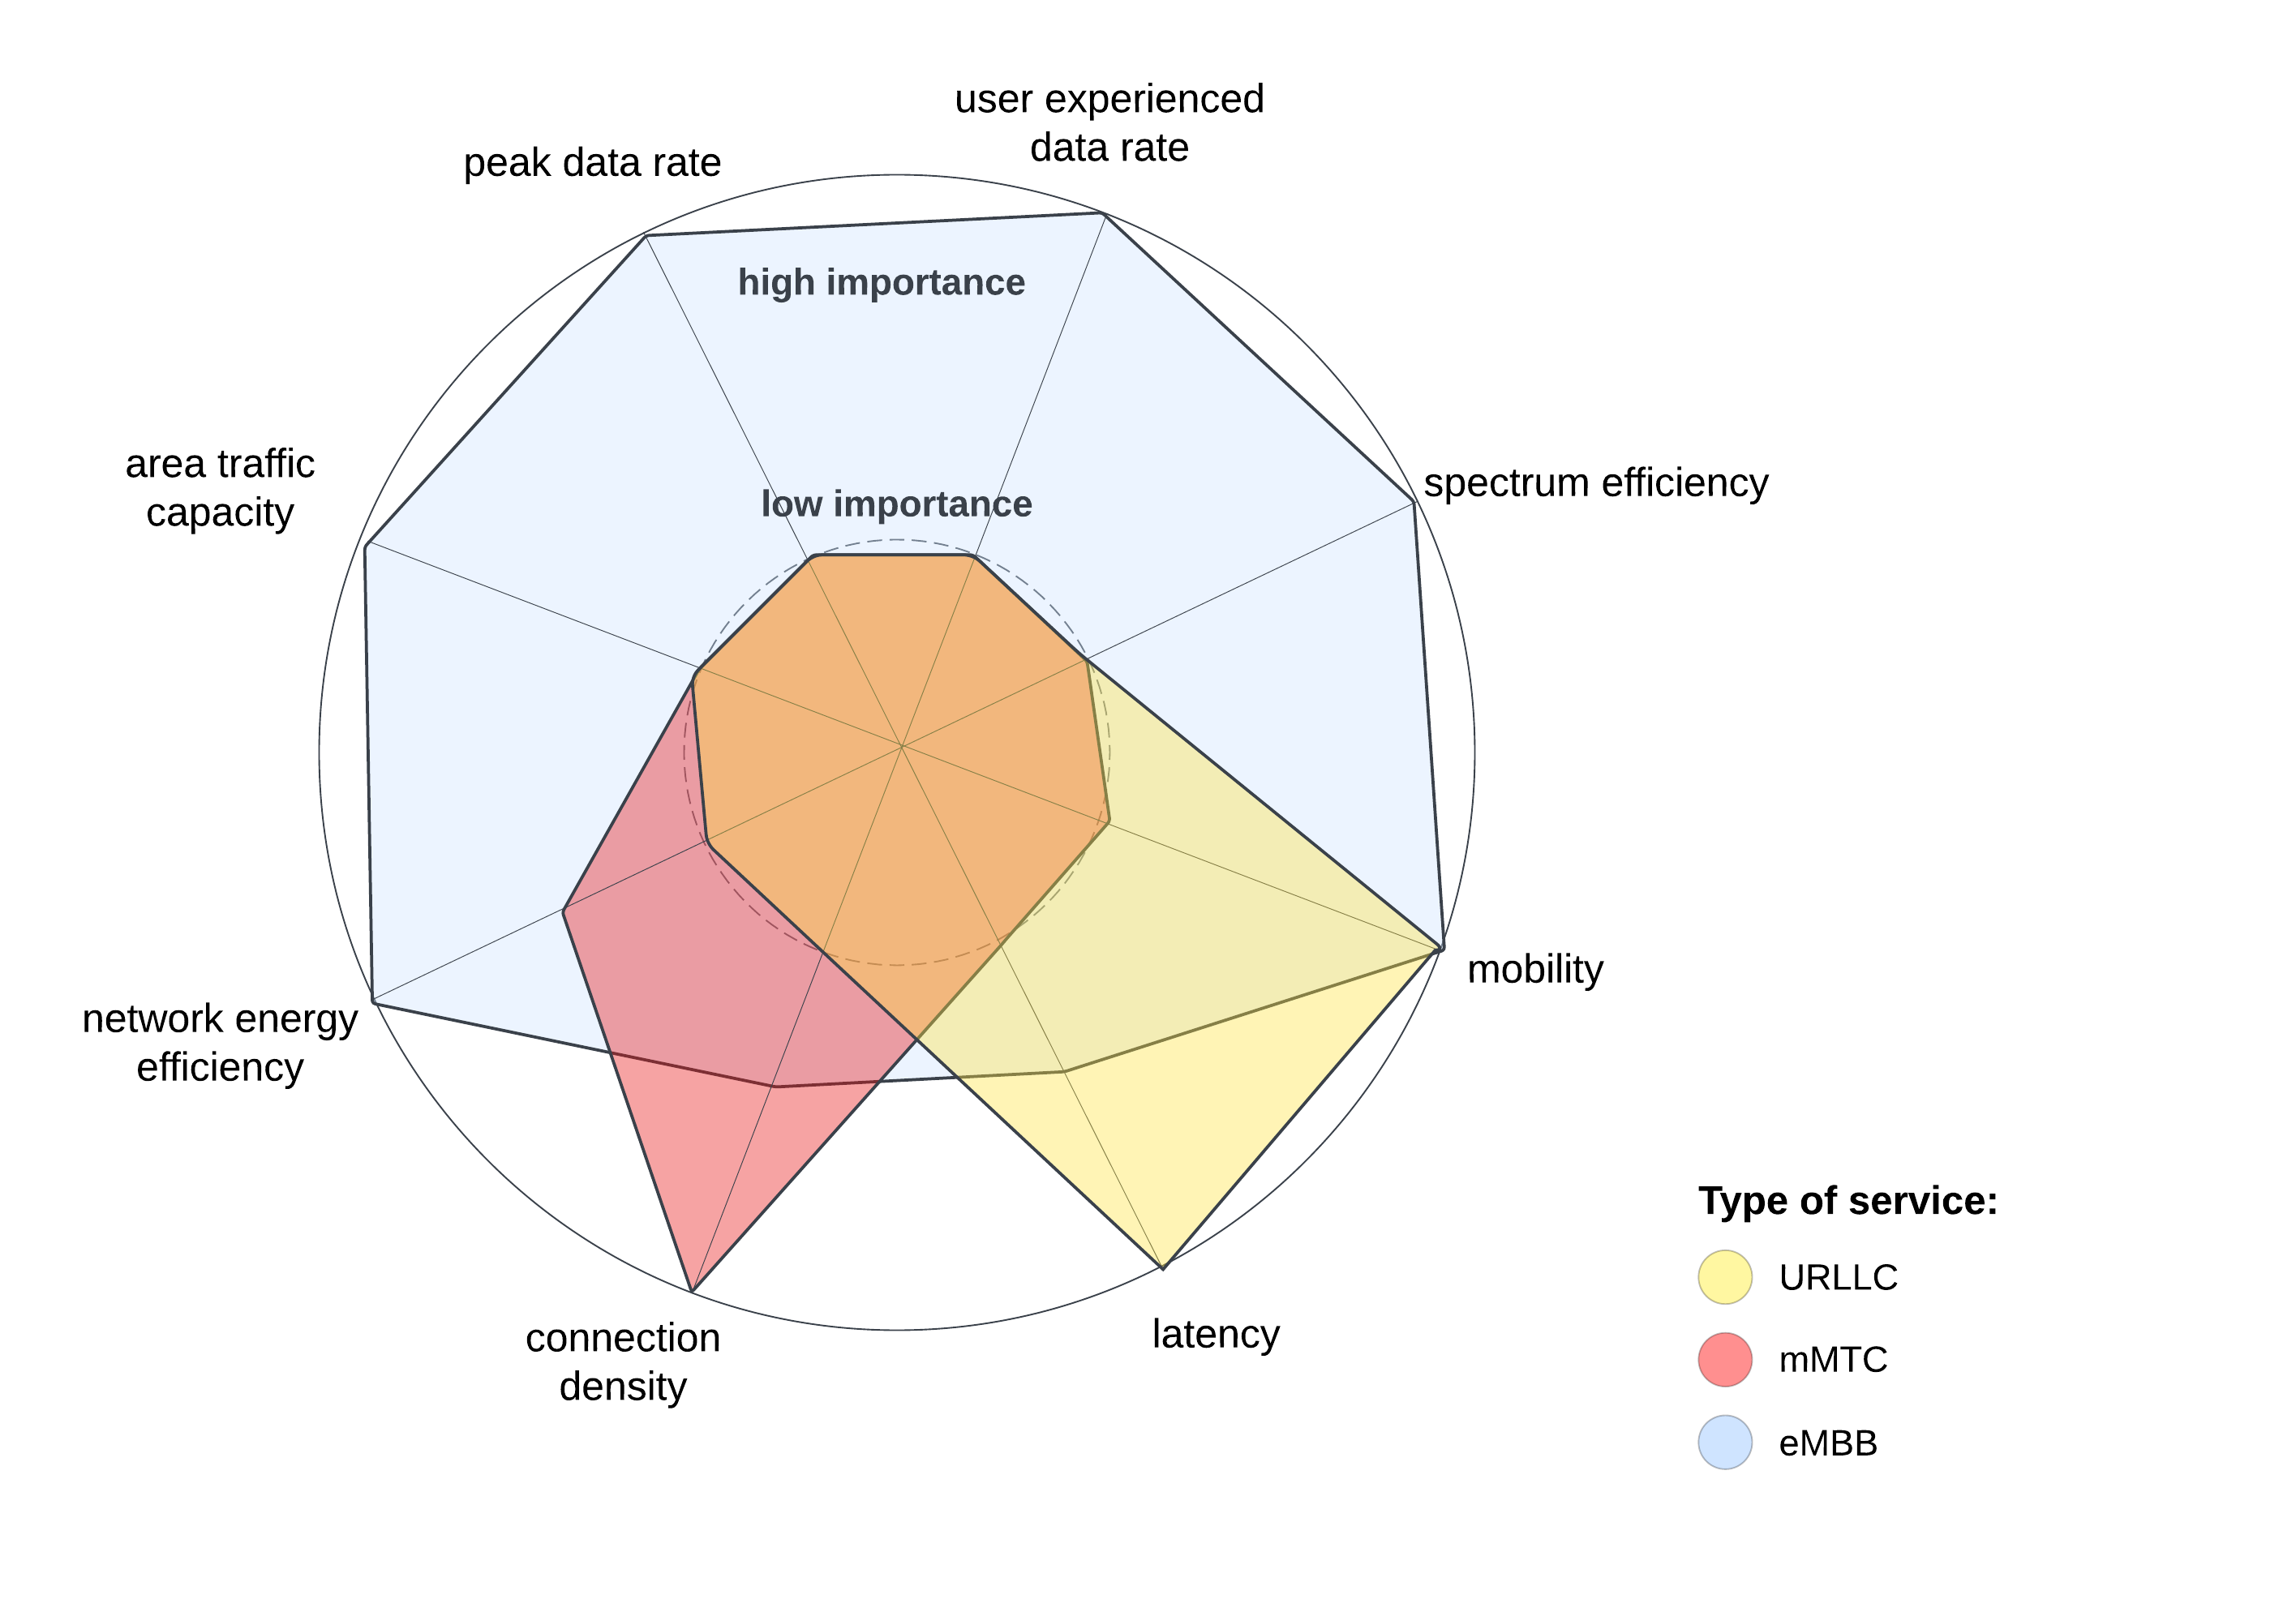
\includegraphics[width=\textwidth]{./images/usage-scenarios.png}
	\caption{My PNG image}
  \end{figure}

As illustrated in Figure [1], the three usage scenarios for 5G are largely varying in their requirements. Trying to cater for all three at the same time would be very inefficient. This leads to the concept of network slicing, i.e., creating multiple logical end-to-end networks on the same physical infrastructure [l]. Each of these logical networks can then be orchestrated individually, according to the specific service requirements [l]. In the context of AVs, this would allow for operation of AVs oriented network slice, which would leverage multiple techniques, even MEC, for achieving low latency. 

The concept of network slicing requires new approaches for managing network resources. The technologies identified as enablers for network slicing are Network Function Virtualization (NFV) and Software Defined Networking (SDN) [l]. NFV aims to leverage virtualization techniques to improve mobile networks’ flexibility, agility and scalability [l]. SDN, on the other hand, aims to provide programmability to mobile networks’ services [l]. 
  
Another important concept, although not new in 5G, is Control and User Plane Separation (CUPS). CUPS allows for distributed CN deployments, where e. g. user plane can be deployed closer to the end user for reduced latency and backbone network traffic. While the user plane solution for both 5G CN and Evolved Packet Core (EPC), the 4G CN, is still quite similar, the control plane underwent a revolution through introduction of Service-Based Architecture (SBA) [k]. The 5G CN Network Functions (NFs) are not connected with point-to-point interfaces, but instead provide Application Programmable Interfaces (APIs) for exposing services to other NFs [k]. In practice, this can be achieved through exposing HTTP REST APIs [d, k]. HTTP (Hyper Text Transfer Protocol) is a request response communication model protocol, while REST (Representational State Transfer) is an architecture style for creating flexible systems that can communicate with each other, using HTTP methods GET, POST, PUT and DELETE. 

\section{5G system architecture}
This section aims to introduce and describe the 5G system architecture with focus on some key NFs, that play role in MEC integration. As described earlier, 5G CN control plane NFs utilize SBA, which means that they are all logically interconnected. The user plane, however, is still connected to the rest of the network using point-to-point interfaces. The 5G system architecture depicted in Figure [2] is described in [m].

\begin{figure}[ht]
	\centering
	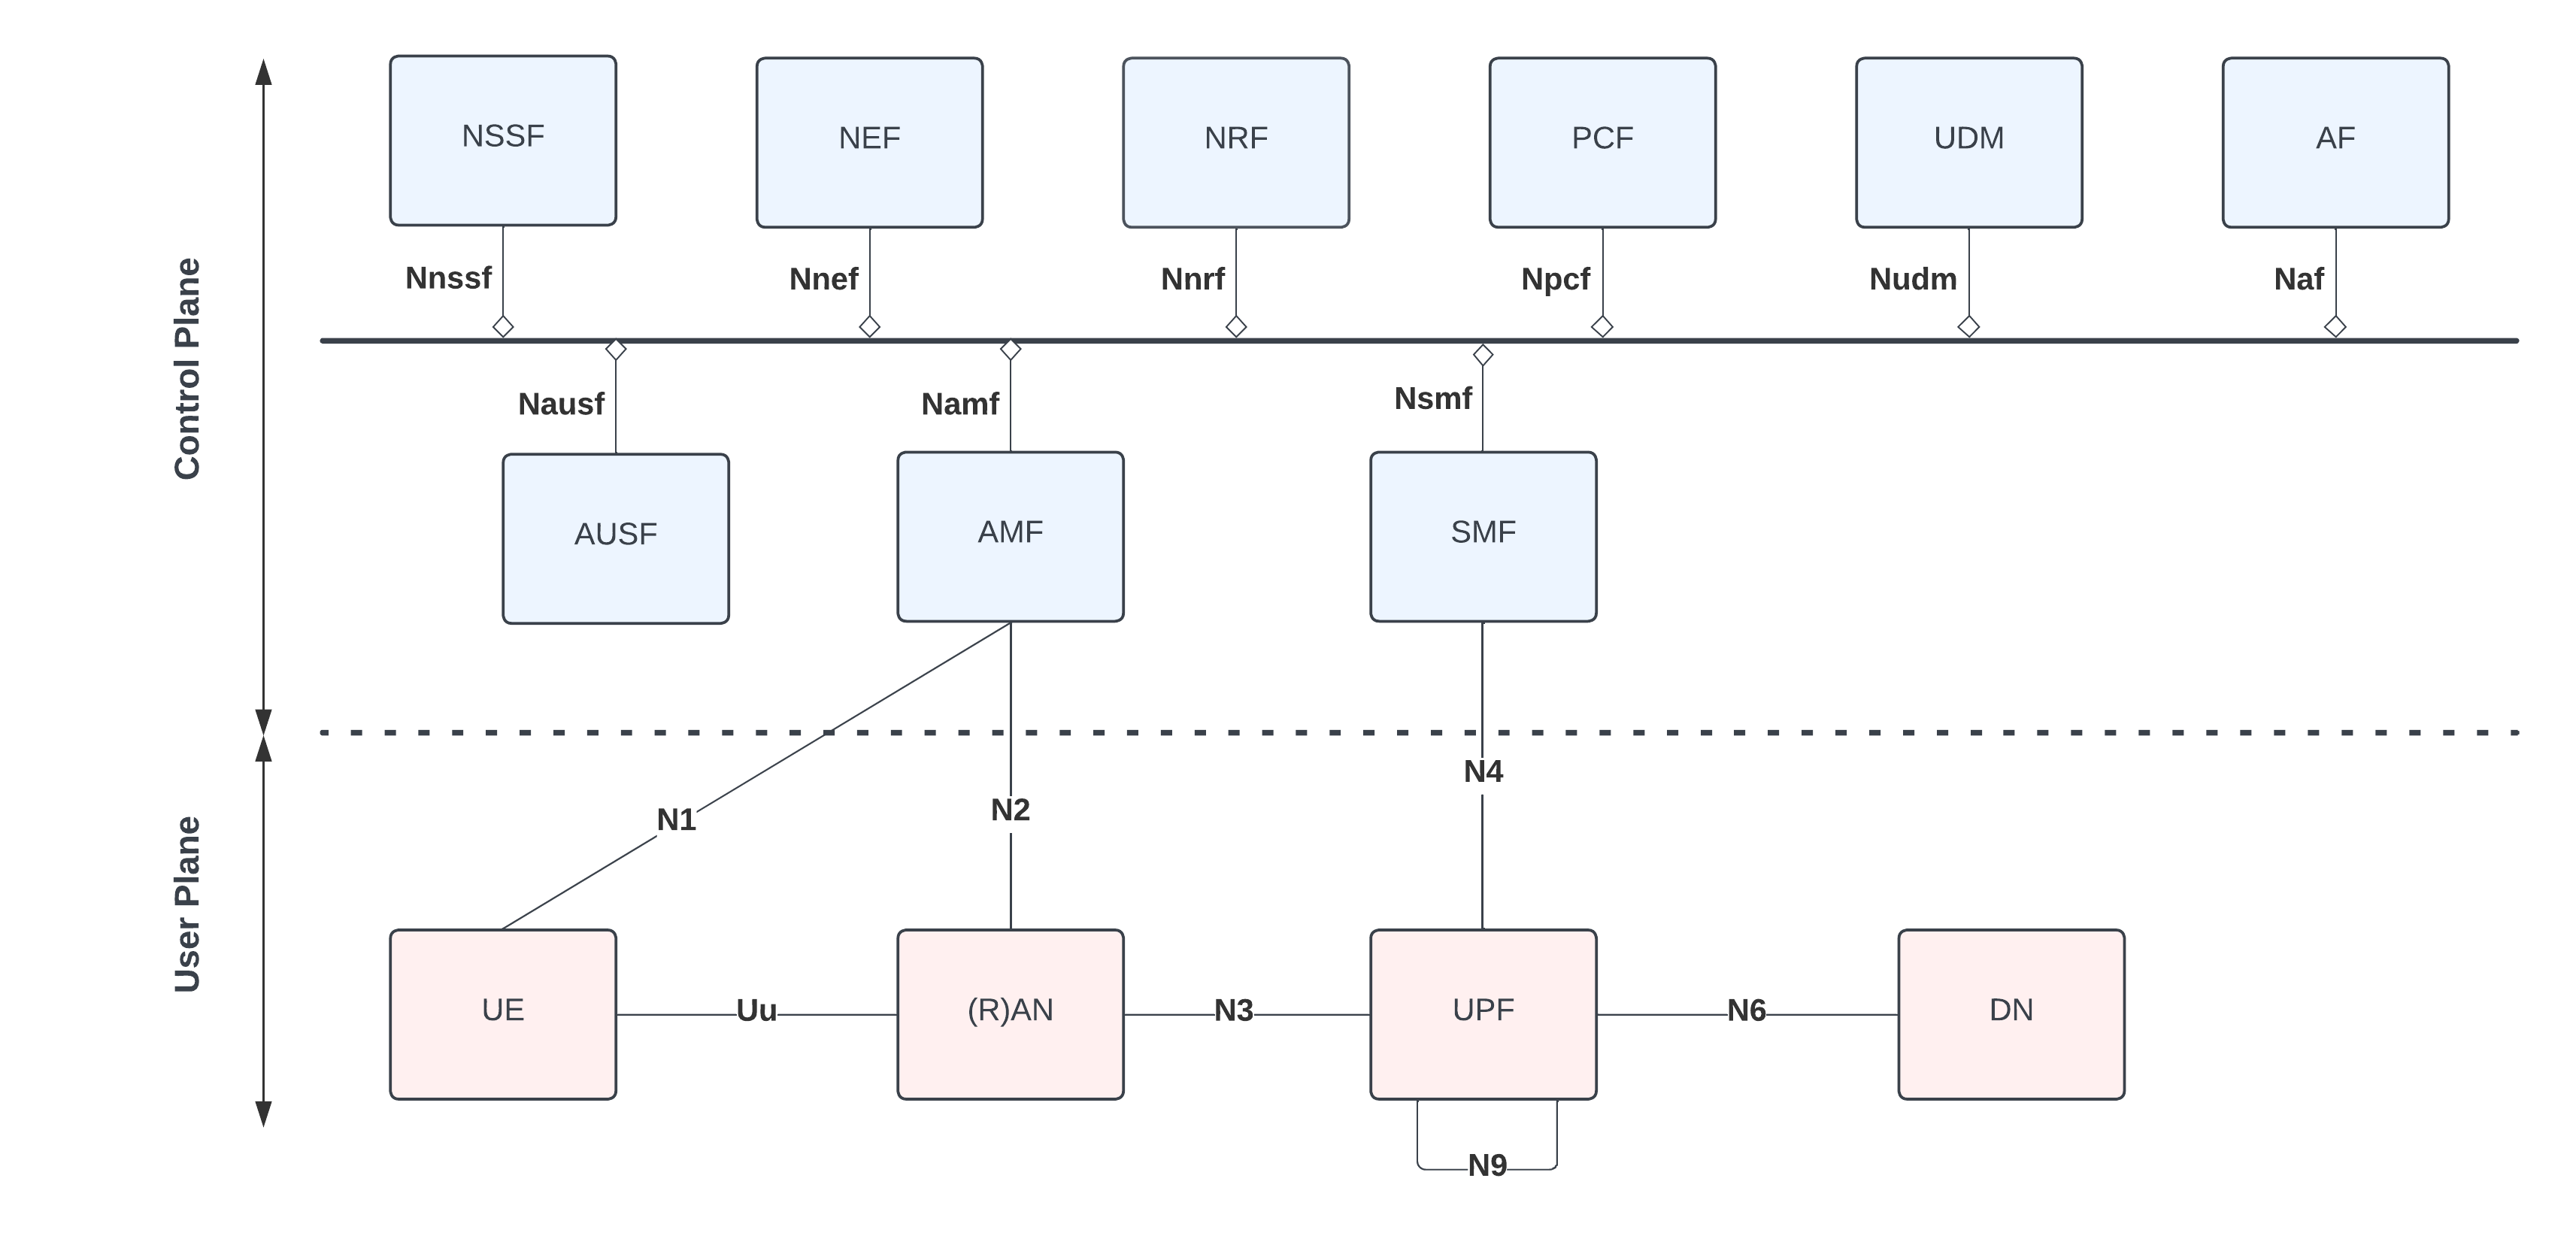
\includegraphics[width=\textwidth]{./images/5G-CN.png}
	\caption{My PNG image}
\end{figure}

The user plane consists of User Equipment (UE), Radio Access Network (RAN), User Plane Function (UPF) and Data Networks Function (DN). The brackets around ‘R’ in RAN in Figure [2] indicate that 5G CN is not designed exclusively for radio access technologies, but instead aims to be access agnostic. UE is connected to RAN via the Uu interface, while RAN itself is connected to the UPF via the N2 interface. The main role of UPF is to process and forward user data. It also connects UEs with IP networks. UPF can be deployed closer to end users, which improves communication latency. This is crucial for MEC deployment, because UPF can be deployed at the network edge with the edge server and steer traffic towards it. [k] 

The control plane consists of Network Slice Selection Function (NSSF), Network Exposure Function (NEF), Authentication Server Function (AUSF), Network Repository Function (NRF), Access and Mobility Management Function (AMF), Policy Control Function (PCF), Session Management Function (SMF), Unified Data Management (UDM) and Application Function (AF). The control plane NFs directly interacting with user plane are AMF and SMF. These NFs together are largely responsible for Packet Data Unit (PDU) session management, initial attach of UE, mobility management or setting up radio bearers. [k] 
  
The AMF deserves special notice, since it is the NF, which acts as a gateway between CN on one side and RAN and UEs on the other. It relays all control signaling messages from other CN NFs towards RAN and UE via the N2 and N1 interfaces. AMF allows UEs to register, authenticate themselves and, in coordination with RAN and other NFs, ensures smooth handover between cells [k]. Although RAN is not extensively discussed in this thesis, it is beneficial to establish how RAN and CN interact to set up communication channels. AMF provides the RAN with Quality of Service (QoS) parameters, which are used by the Radio Resource Control (RRC) protocol to set up appropriate radio bearers, i.e., logical radio connections between UEs and RAN [a]. 
  
An important workflow, key to understanding how MEC can be integrated to 5G system, is PDU session management of 5G system, which  provides connectivity between UEs and DNs, mostly the Internet. To set up this connection, UE sends a PDU session establishment request to AMF, which instructs SMF. What follows is a series of control plane signaling messages between SMF and various other NFs to properly register the PDU session, set up (R)AN and create a UPF tunnel towards the DN. The simplified PDU session establishment process is illustrated in Figure [3]. 5G system architecture allows for the UE to be to be connected to multiple DNs at a time. One PDU session can connect the UE to the Internet, while another one can be set up to connect it with, e.g., local edge server. To determine the correct endpoint DN for a given traffic, UPF uses an Uplink Classifier (Ul CL), which enables steering traffic towards appropriate DNs based on, e.g., uplink IP address. Crucially, configuring UL CL can be requested by AF as a SMF service. [k] 

\begin{figure}[ht]
	\centering
	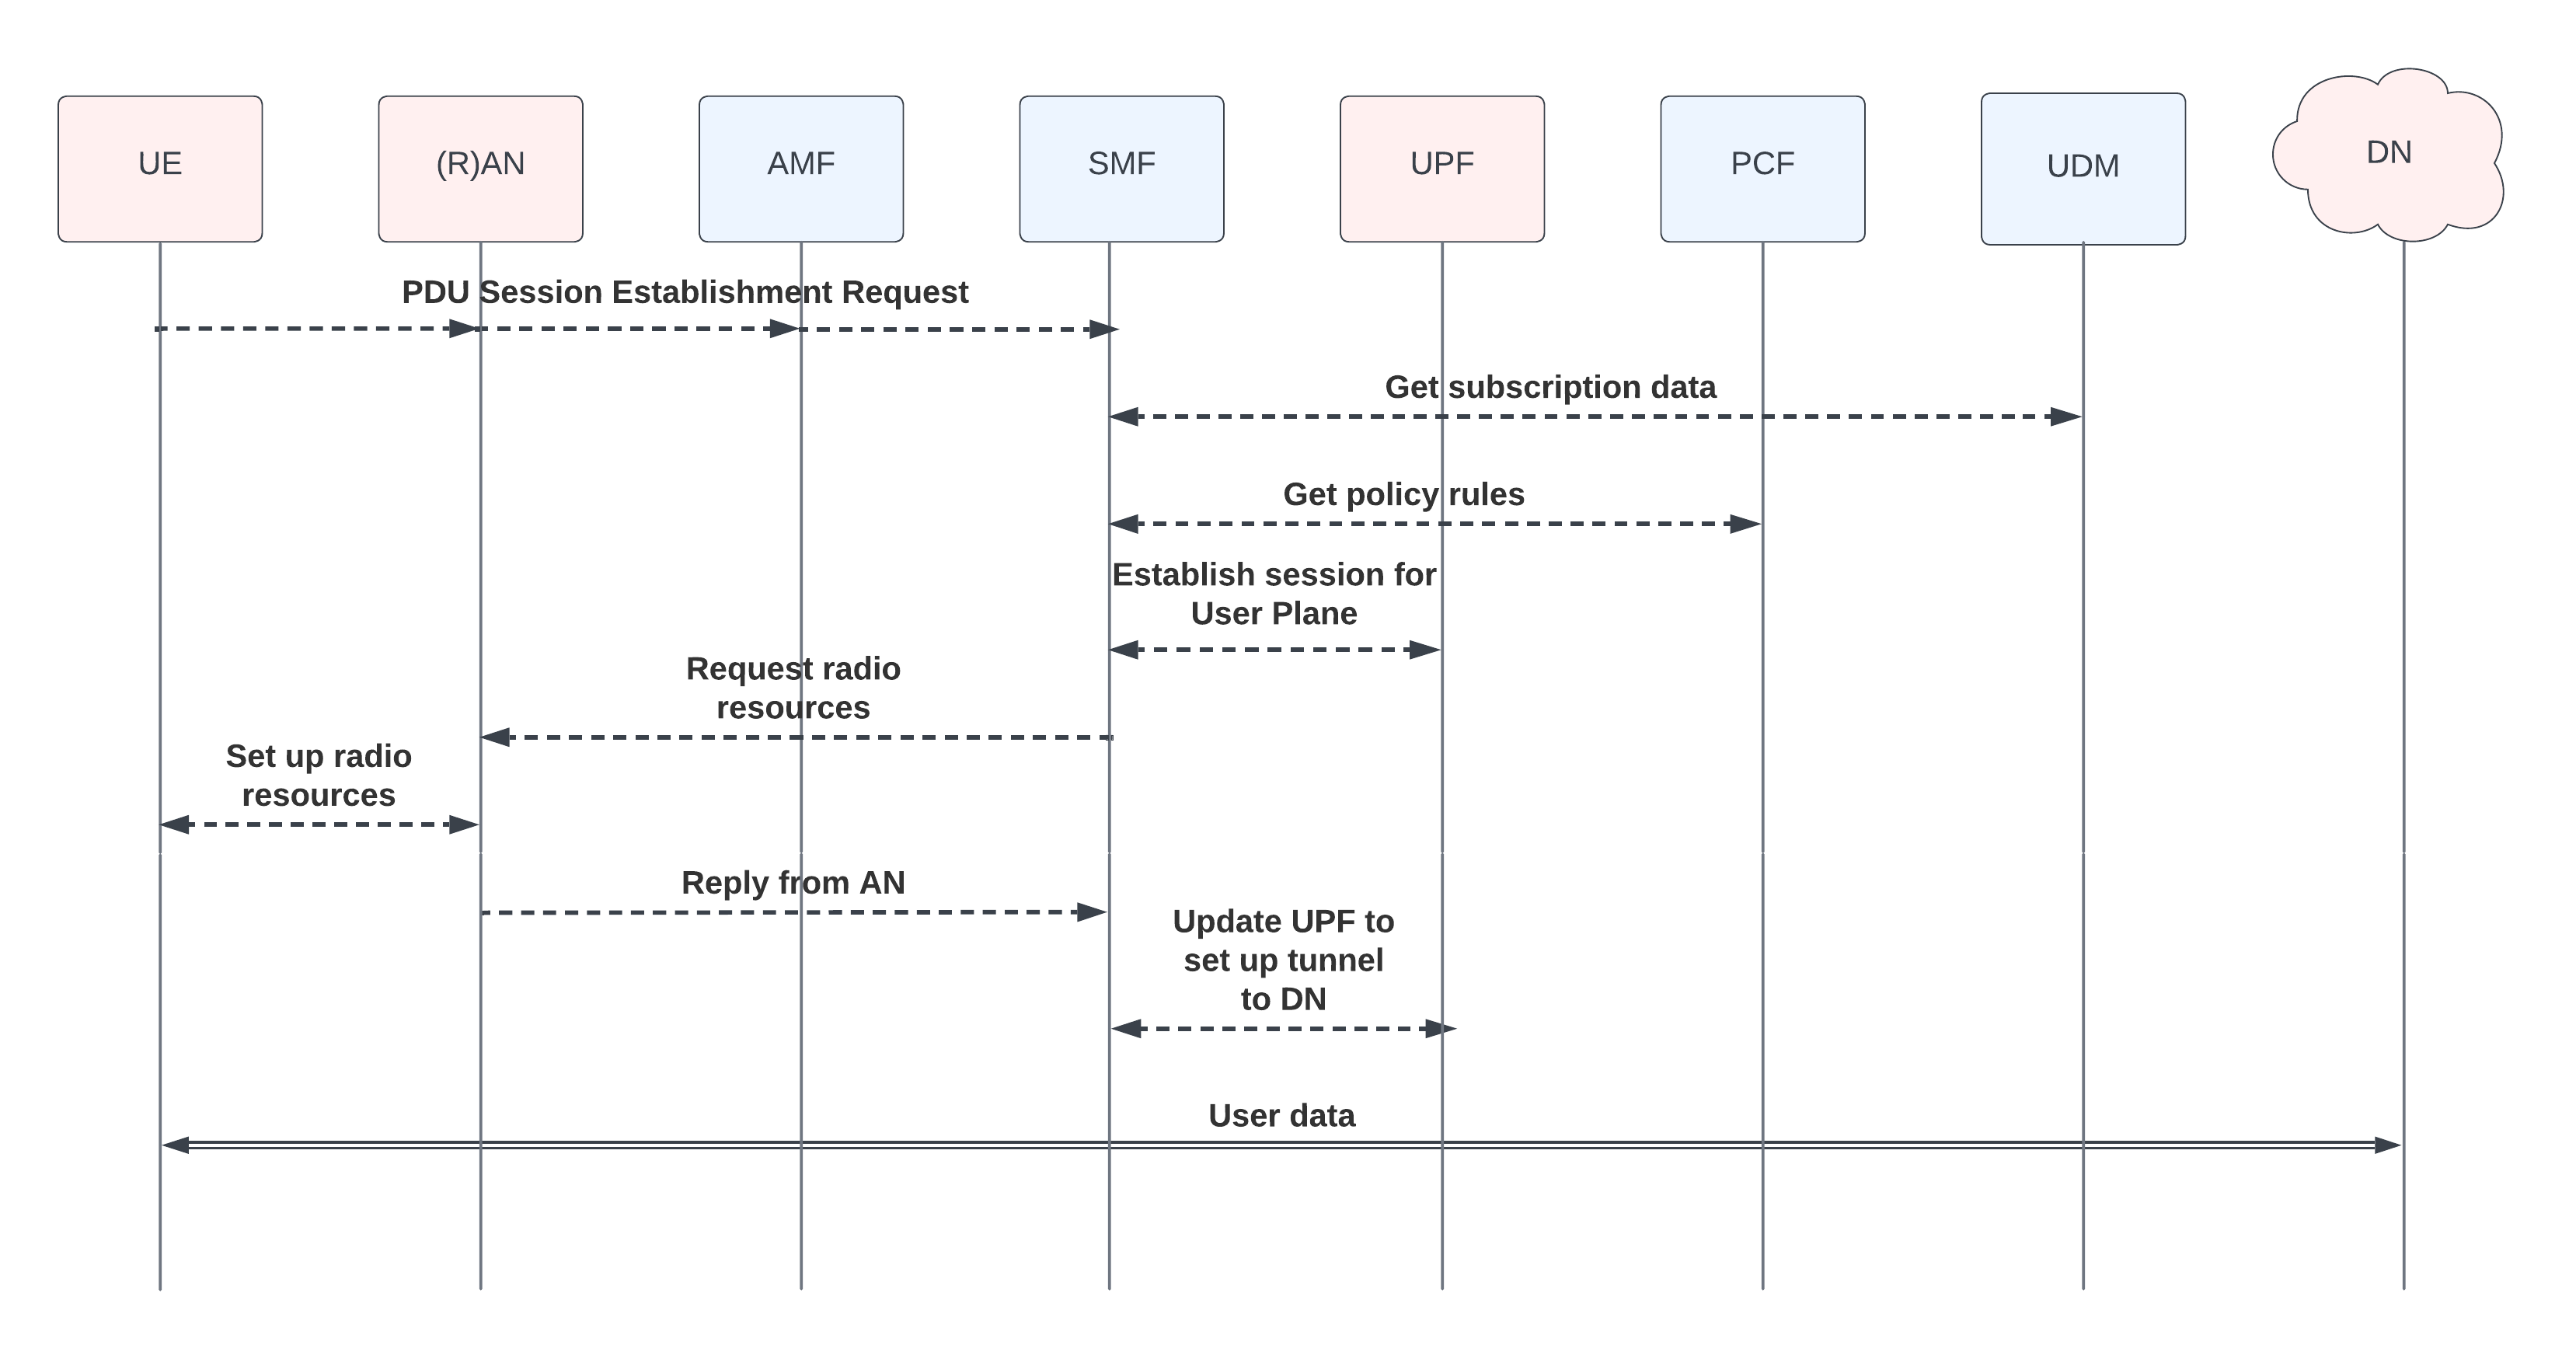
\includegraphics[width=\textwidth]{./images/PDU-sesh-est.png}
	\caption{My PNG image}
\end{figure}

The PDU session management was slightly innovated, compared to 4G. 5G system, however, introduces completely new workflows: service registration \& discovery and capabilities exposure. These workflows are crucial for understanding how 5G system interacts with external applications such as MEC. Service registration \& discovery, illustrated in Figure [4], describes how individual NFs within 5G system utilize the SBA to provide and consume services. Put simply, every Service Producer needs to register its services with NRF. When a Service Consumer wants to request services of a particular NF, it first requests NRF for a list of available NFs offering those services. The other workflow, capabilities exposure, describes specifically how external applications can interact with and influence 5G system. The NFs crucial for this workflow are AF, which basically represents the external application, and NEF, which acts as a gateway between external applications and 5G system. Provided the external application is properly registered, NEF can e.g. allow AF to influence traffic steering, managed by SMF, to forward traffic to a specific DN. This is of particular interest to MEC integration, since this workflow can allow MEC to influence traffic steering from UE to edge server. This flow is illustrated in Figure [5].

\begin{figure}[ht]
	\centering
	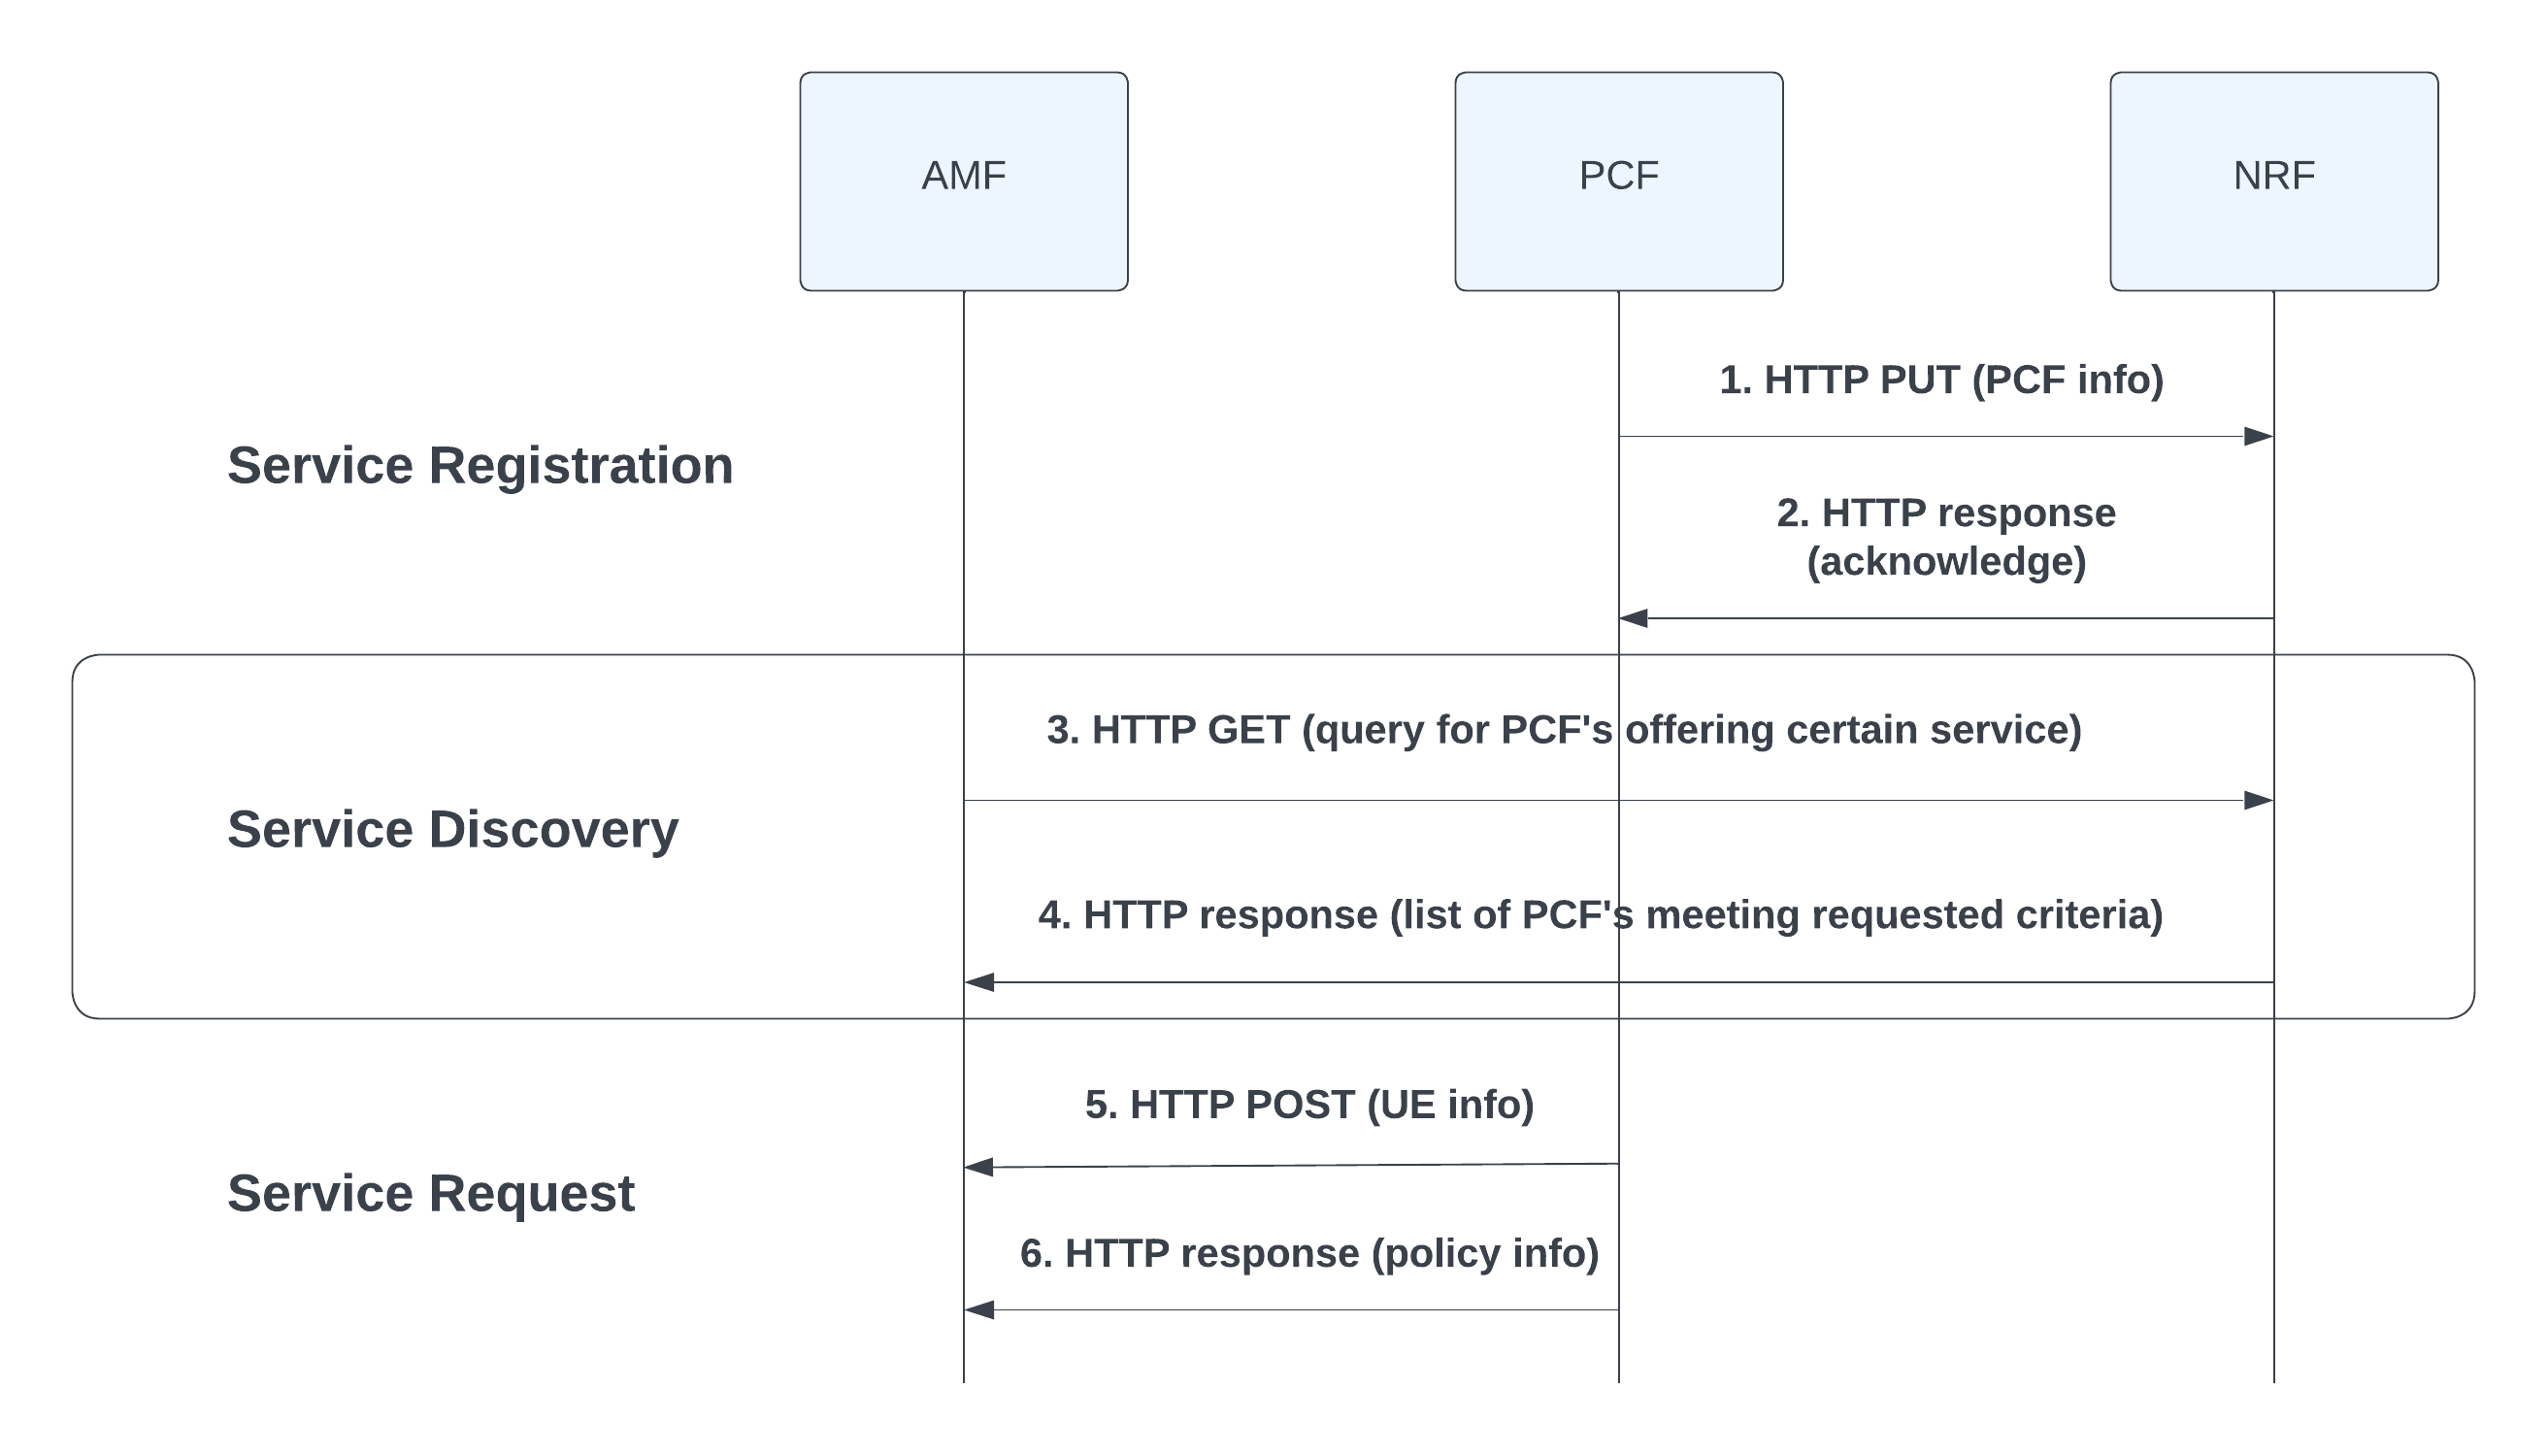
\includegraphics[width=\textwidth]{./images/5G-reg-disc.png}
	\caption{My PNG image}
\end{figure}

\begin{figure}[ht]
	\centering
	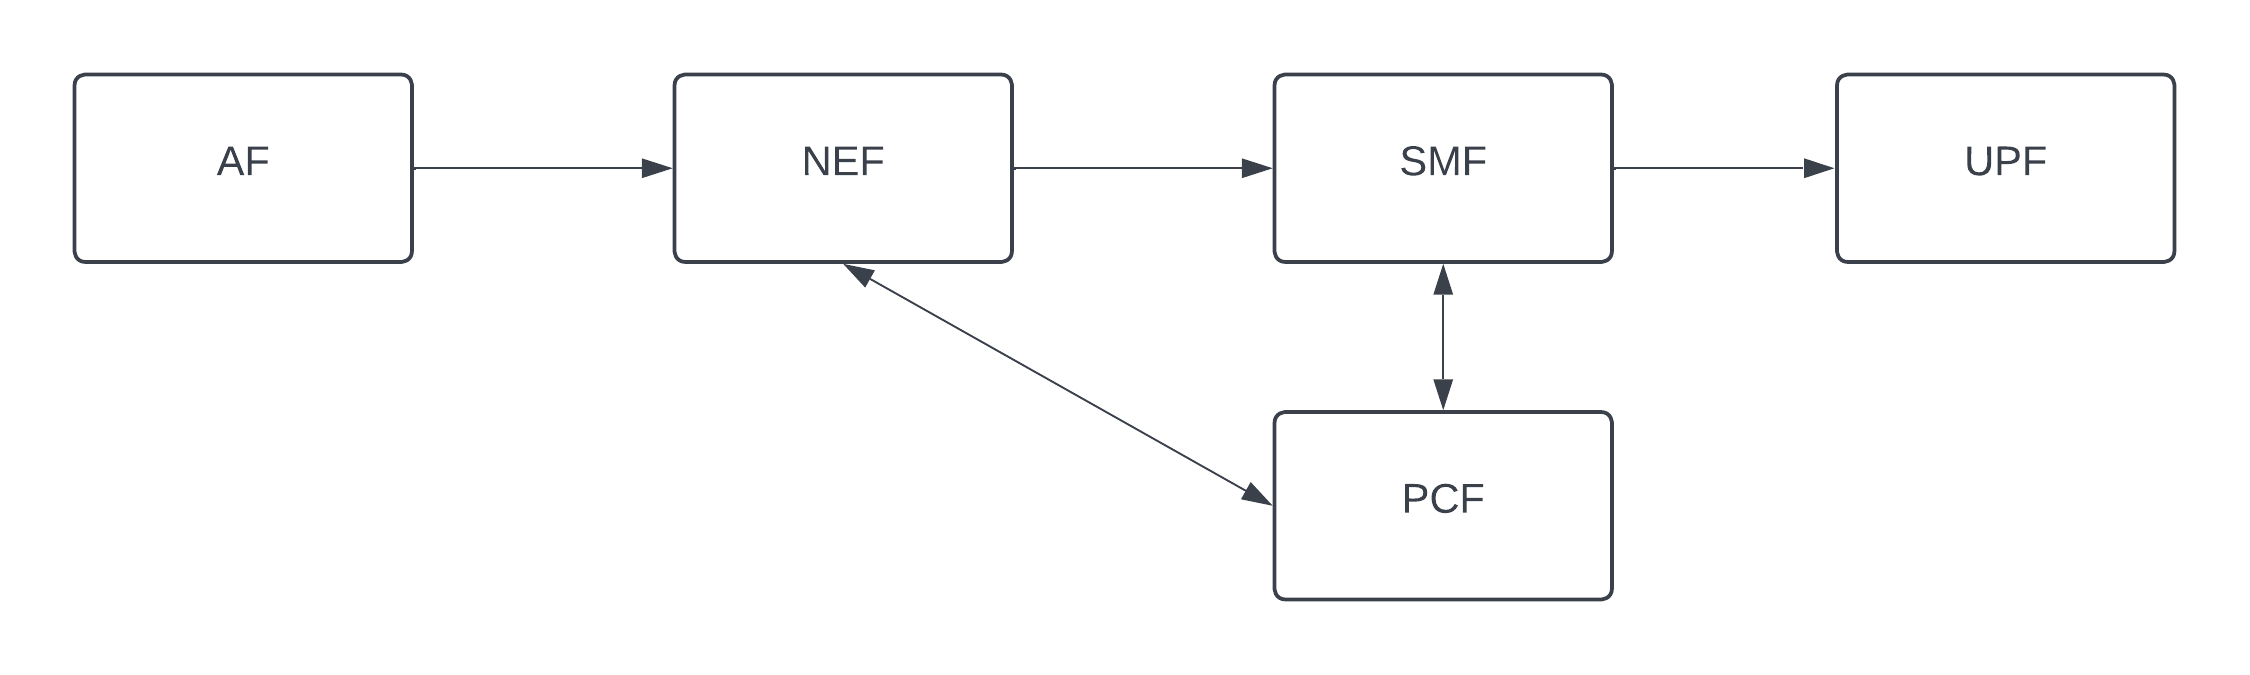
\includegraphics[width=15cm]{./images/traffic-control.png}
	\caption{My PNG image}
\end{figure}

\section{MEC system concept and architecture}
Previous sections of this chapter focused on providing a general overview of the 5G system, as well as identifying individual workflows supporting MEC integration. This section switches the focus to the MEC system itself and aims to, again, provide a general overview before selecting key functional entities (FEs) and workflows that play a role in connecting the MEC system to a 5G mobile network. 

The general idea of MEC is to bring CC capabilities to the network edge and thus provide a low latency environment for improved experience in existing applications and for enabling emerging applications in industrial IoT or automotive sectors [n]. This would open the 5G ecosystem to new vertical sectors and enable exploitation of new business opportunities [d]. However, having multiple stakeholders in the development chain of end-to-end MEC solutions implies the need for standardization [n]. MEC standards play an important role in creating a common platform for Mobile Network Operators (MNOs) and MEC application developers from various verticals to aid the development of end-to-end MEC solutions. This section presents and describes the MEC system framework and reference architecture developed by ETSI ISG MEC, the leading standardization body in MEC. 

The MEC framework, defined in [j], is illustrated in Figure [6], which shows the general entities involved and groups them into system level, host level and network level FEs. The network level entities ensure connectivity to local area networks, cellular networks and external networks, e.g., the Internet. The host level, constituted by MEC host and its management, is the core of MEC system, because it represents the IT infrastructure on which MEC applications (MEC apps) are run. The MEC host can be further dissected into MEC platform, virtualization infrastructure and MEC applications [j]. The system level is responsible for management and orchestration of the whole MEC system, which is typically comprised of multiple MEC hosts [j, d].

\begin{figure}[ht]
	\centering
	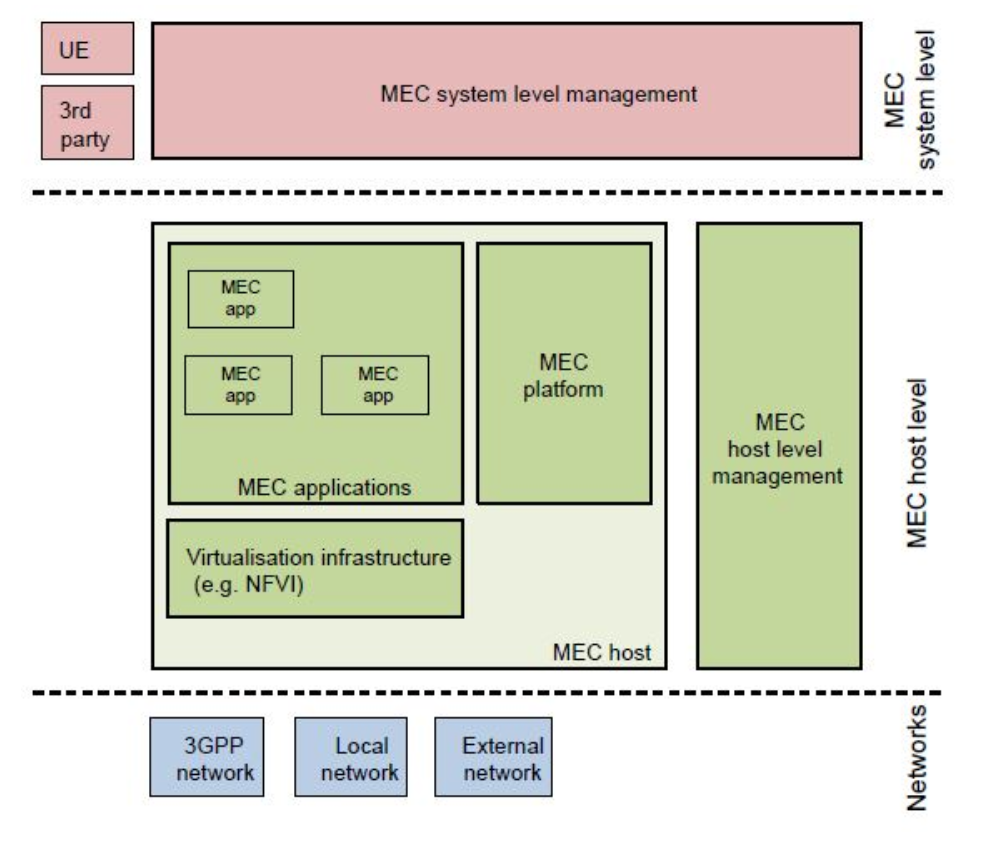
\includegraphics[width=\textwidth]{./images/MEC-framework.png}
	\caption{My PNG image}
\end{figure}

The reference architecture, illustrated in Figure [7], offers a more detailed insight into the general framework from Figure [6] and identifies reference points for connecting individual FEs of the MEC system. The reference points can be divided into three groups based on [j]: 
\begin{itemize}
	\item MEC platform functionality reference points (Mp) 
	\item Management reference points (Mm)
	\item Reference points connecting to external entities (Mx)
\end{itemize}
Not all the illustrated reference points are specified by ETSI ISG MEC [j]. An example of a specified interface is the Mp1, connecting MEC Platform and MEC apps. This is desirable since it is expected that MEC platform and MEC apps will be developed by different parties. An example of a closed interface is the Mm5, connecting MEC platform and its management entity, which are both expected to be developed by the same organization and are therefore left as an implementation choice [j, d].

\begin{figure}[ht]
	\centering
	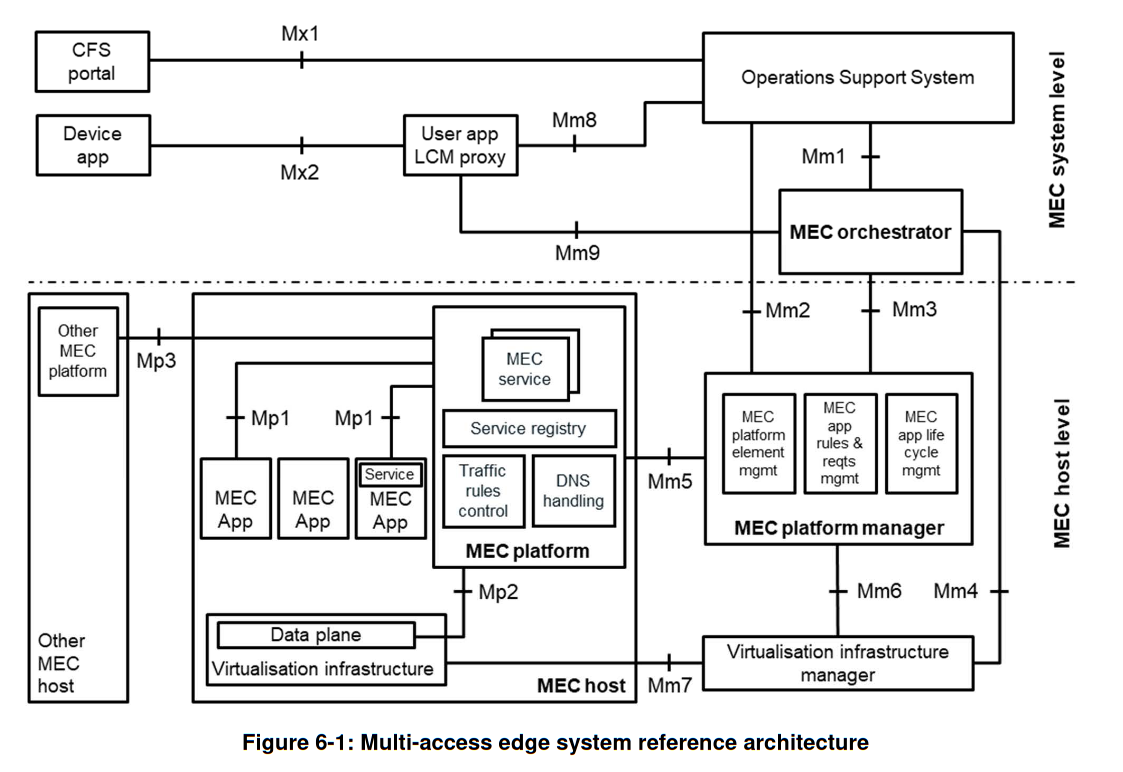
\includegraphics[width=\textwidth]{./images/MEC-ref-arch.png}
	\caption{My PNG image}
\end{figure}

The MEC platform is a crucial MEC system FE, as it acts as an intermediary between MEC apps and the system level management. Through the Mp1 interface, MEC platform offers an environment where MEC apps may discover, advertise, consume and offer MEC services [o]. This is very similar to the SBA based workflows in 5G system. MEC platform offers the MEC apps similar functionality to what NEF and NRF offer to the 5G system. On top of that, the MEC platform has another very important responsibility. Upon request from a MEC app, MEC platform can activate, deactivate or update traffic rules and then configure the data plane accordingly [j]. This in turn is analogous to AF functionality within 5G system. These analogies are elaborated upon in the next section focusing on integration of MEC system to 5G mobile network. 

Another important part of the MEC system is its management, split into host level and system level, which is illustrated in Figure [6]. The individual FEs taking part in MEC management are illustrated in Figure [7]. System level management is comprised of Operations Support System (OSS), User Application Life Cycle Management Proxy (UALCMP) and MEC orchestrator (MEO). MEO is a key FE overseeing the whole MEC system in terms of deployed MEC hosts, available resources and services etc. It also plays a key role in application onboarding or mobility handling. Host level management responsibilities are shared between two entities: MEC Platform Manager (MEPM) and Virtualization Infrastructure Manager (VIM). MEPM manages lifecycle of applications and can inform MEO about MEC app related events, while VIM prepares the virtualized resources of the virtualization infrastructure. [j] 

Thus far, it has been described how MEC apps and MEC platform interact with each other to provide and consume services and how the whole MEC system is managed on both system and host levels. The last important workflow to be described is how the MEC system interacts with the UE, so that the UE can discover and exploit available MEC servers.  There are two recognized approaches for edge discovery from the UE perspective: DNS based and device based [n]. The first option is called edge unaware, since the client application, i.e., the application instance in UE communicating with MEC app, has no information about the edge server location. Instead, the client application is connected to the MEC app via a DNS server, whose queries may be enriched by the 5G CN with the device location information [n, p]. The second approach, edge aware, requires a new entity on the client side, the device application, to communicate with the MEC system to receive the MEC application address and offer it to client applications [p]. The edge aware approach is more suited for highly distributed edge cloud exposed to UE mobility, because it allows for informing the device application about change of edge server [n]. In stateful applications, this requires the MEO to trigger context migration to another server [j, n].

\section{Integration of MEC into 5G system}
The previous sections of this chapter provided a brief overview of both 5G system and MEC system respectively with focus on techniques and concepts that can be used for their seamless integration. This section aims to deliver an end-to-end framework for MEC and 5G integration based on standards by 3GPP and ETSI MEC. This is of vital importance for the rest of the thesis, but it can also be valuable for developers of MEC solutions. 

The lifecycle of a MEC app can be divided into four stages, based on [p]:
\begin{itemize}
	\item MEC app packaging and onboarding
	\item MEC app instantiation 
	\item Client-side app and MEC app communication 
	\item Usage of the MEC platform and services 
\end{itemize}
MEC apps are expected to be packaged in Virtual Machines (VMs) or containers and to run on the virtualized infrastructure of a MEC host. The onboarding of MEC apps is left as an implementation choice for the MEC operator [p]. The second stage of a MEC app lifecycle describes how it is instantiated on a MEC system and how it is made available to clients. There are two options for a MEC app initialization and, eventually, for establishment of communication between the client-side app and the MEC app. One option is via a communication between the device application and the MEC system through a UALCMP, and the other is via the OSS without the need for any client-side action. The first option is related to edge-aware discovery, described in previous section. Device application contacts the UALCMP via the Mx2 interface and informs it which MEC app it would like to instantiate, the UALCMP then informs the MEO, which is responsible for choosing the appropriate MEC host and configuring the MEPM to initialize the given application. In response to successful instantiation, the device app receives the IP address of a running MEC app instance [p]. In the other option, the initialization is done without the client-side being required to participate in the process. For the client app, to utilize MEC, it simply accesses the required application via its domain name and the 5G system DNS is responsible for connecting the client to the nearest running MEC app instance [n, p]. Once instantiated, MEC apps can leverage SBA within the MEC system, consuming services provided by the MEC platform or other applications and also offering their services to other applications. 

Thus far, it has been hinted that EC can be exploited in two varying ways, both of which end in the UE accessing the desired application in an edge server to experience low latency. The simpler option, relying on DNS servers connecting clients to the nearest edge server, requires less effort to implement but it has several limitations. It is less suited for highly mobile scenarios and highly distributed cloud [n]. The second option relies on tight integration of the MEC system and the underlying mobile network. As a result, it offers better support for highly mobile scenarios, even allowing for context migration between MEC app instances in stateful applications. On top of that, MEC offers a framework for MEC apps, through which they can feed traffic rules to the mobile network to help satisfy QoS requirements. This is achieved through establishment of a dedicated PDU session steering traffic from the client app to the MEC host. 

The resulting framework, utilizing edge aware app initialization and dedicated PDU session establishment is as follows: 
\begin{enumerate}
	\item Device app requests initialization of a MEC app from UALCMP
	\item MEO chooses the optimal MEC host and sends traffic rules to the selected MEC platform
	\item MEC platform, acting as an AF, requests traffic rules control from SMF, via NEF/PCF 
	\item SMF configures the UPF with UL CL to steer desired traffic to MEC host
\end{enumerate}

\begin{figure}[ht]
	\centering
	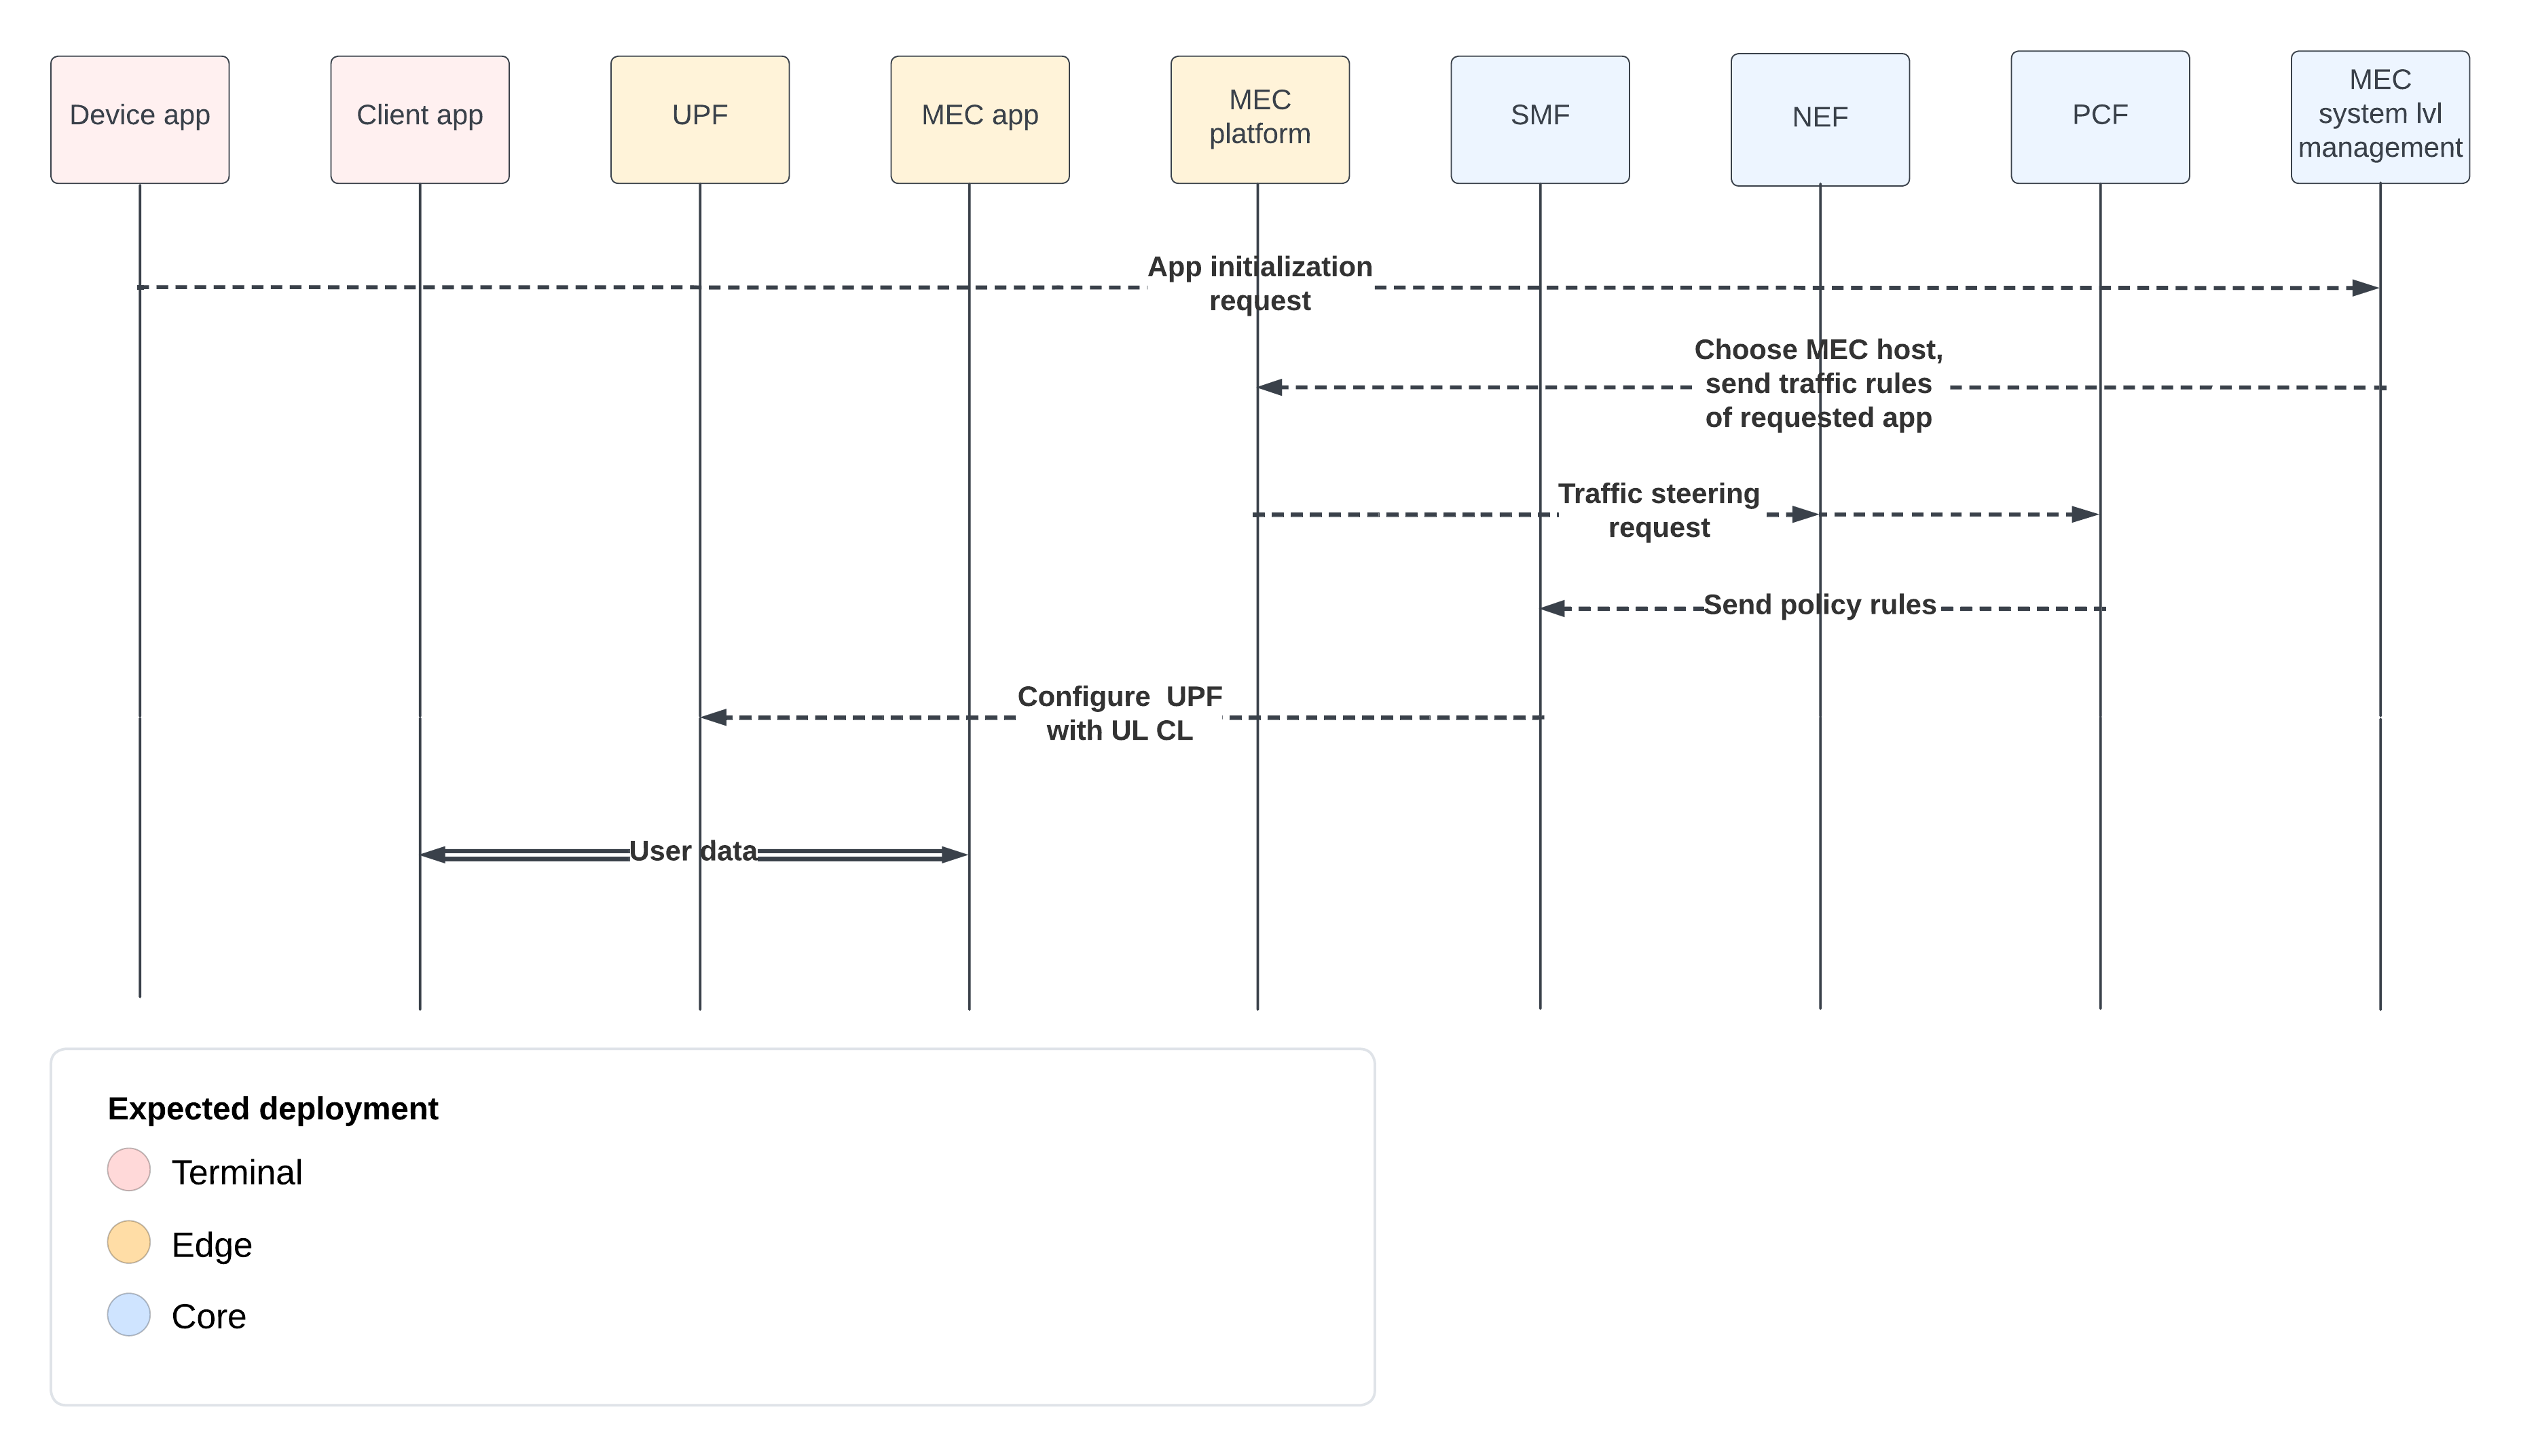
\includegraphics[width=\textwidth]{./images/MEC-5G-integration-flowchart.png}
	\caption{My PNG image}
\end{figure}

\chapter{Open-source MEC Solutions}
\label{ch:o-sMEC}
This chapter introduces the rich and growing ecosystem of open-source MEC solutions with the goal of eventually choosing the most suitable project to leverage in the development of VEC testbed. The world of open-source MEC solutions has developed from the need to accelerate the development process of MEC applications and to support the adoption of MEC as a key technology within 5G mobile networks. The resulting environment comprises of various MEC projects, developed by a range of stakeholders, addressing different challenges within MEC. This chapter intends to describe the open-source MEC ecosystem by introducing the main bodies taking part in MEC development, their respective projects and the challenges these projects aim to address. 

The main criteria studied in evaluated MEC projects are which part of the ETSI MEC system they aim to constitute and what underlying technologies they use. Another important factor is interoperability support, i.e., which interfaces are provided in the project to enable communication with modules developed by different stakeholders. An end-to-end MEC solution is expected to be developed by three stakeholders: MEC app developer, mobile network operator and MEC operator. The evaluated open-source projects play the role of a MEC operator. Therefore, it is crucial that they provide means of integrating it with both MEC apps and mobile networks. Furthermore, all the evaluated projects are a work in progress, they may not yet provide all the desired functionality or may not be fully operational. Therefore, some promising projects were tested and their state of operationality will be discussed. 

Before evaluating the individual projects, it is desirable to mention the most often used software techniques leveraged in these projects. The most important one is virtualization. In the previous chapter, it was described how the architecture of both 5G network and MEC system consists of several building blocks called NEs or FEs. These building blocks are not implemented by specific hardware parts, instead, the trend is moving towards virtualization, i.e., managing multiple separated software-defined entities on general hardware. The way in which the separation is achieved sets apart different virtualization techniques. One way is to introduce a new abstraction layer on top of the hardware – the hypervisor, then the separation is created by having multiple Virtual Machines (VMs) with their own operating system running on top of the hypervisor. Another way is to package the desired application and all of its dependencies in blocks called containers. All running containers share the same underlying operating system and are thus a significantly more lightweight solution than VMs. 

Some popular hypervisors are VirtualBox or VMware and the most common platform for container virtualization is Docker. Orchestrating multiple containers on a single node is often handled by Kubernetes (k8s), a popular open-source container orchestration tool. Another key software, Open vSwitch, provides virtual networking layer for VMs or containers and enables their connectivity to each other and to data networks.

\section{Akraino projects}
The leader in development of open-source edge software is LF Edge, a Linux Foundation umbrella organization, which aims to unite industry leaders to introduce edge computing framework. LF Edge identifies three levels of maturity within their projects. Only two projects are, at the time of writing, listed in the top category: Akraino and EdgeX Foundry [q]. The latter, EdgeX Foundry, has established itself as the leading open-source industrial IoT edge framework. Akraino, on the other hand, spans over a broad variety of use cases, including but not limited to MEC. Akraino is not one common platform, but rather a whole set of edge stack solutions, called blueprints. Furthermore, in 2019 LF Edge signed a cooperation agreement with ETSI, which lead to an increasing number of Akraino blueprints tightly following ETSI ISG MEC specifications [d]. Under the newest – sixth release, Akraino constitutes of over 30 blueprints, such as: Connected Vehicles Blueprint (CVB), Enterprise Applications on Lightweight 5G Telco Edge (EALTEdge) or Public Cloud Edge Interface (PCEI) [q].
\subsection{Connected Vehicles Blueprint}
The CVB blueprint is developed by Tencent, Arm, Intel and Nokia. It aims to create a MEC platform offering services to connected vehicles. Some applications running on top of the provided platform include traffic situation monitoring, road event perception or high precision positioning. It references the ETSI MEC Mp1 and Mm5 interfaces, which are supposed to handle communication between MEC platform, MEC platform management and MEC apps. It is not uncommon among MEC solutions to leverage some related open-source software, CVB uses StarlingX as a virtualization platform, TARS as a microservices management tool and OpenNESS toolkit for managing and onboarding edge services. The setup of CVB requires three nodes: Jenkins master, TARS master and TARS node with the vehicle applications. An illustration of the scope of CVB is shown in Figure 9. [r]
\begin{figure}[ht]
	\centering
	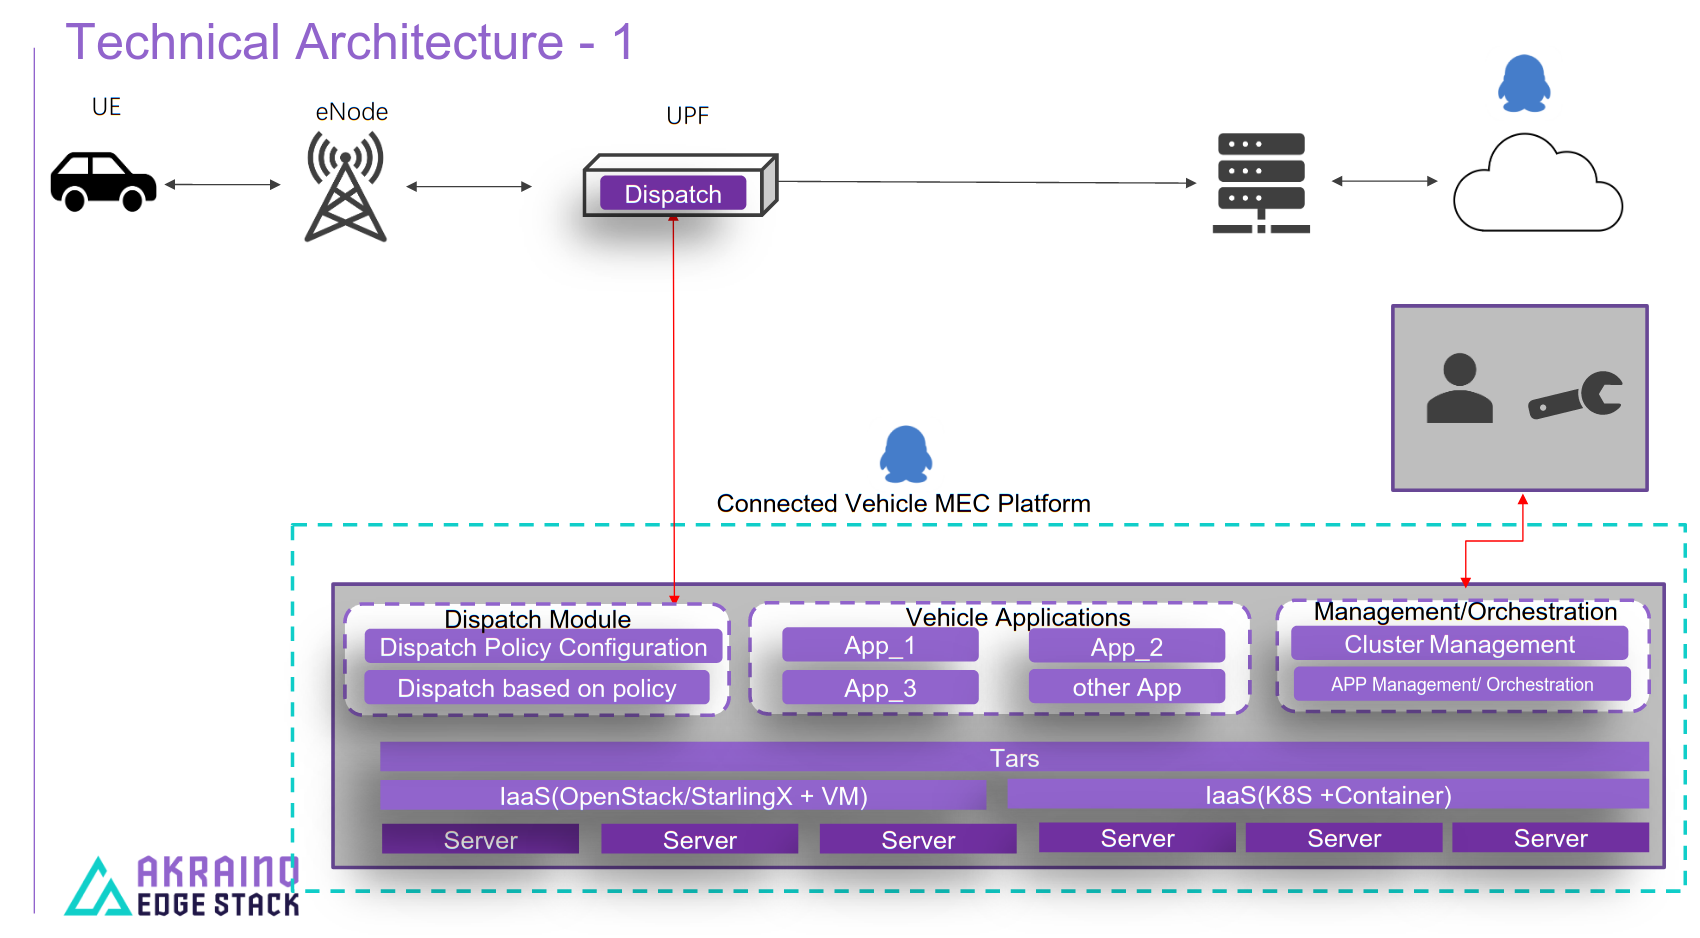
\includegraphics[width=\textwidth]{./images/akraino-cvb.png}
	\caption{My PNG image}
\end{figure}

\subsection{Enterprise Applications on Lightweight 5G Telco Edge}
EALTEdge is a blueprint under 5G/MEC system blueprint family within the Akraino project. It is intended to play the role of a MEC operator through offering MEC platform as well as its management and orchestration to host enterprise applications on lightweight 5G telco edge. EALTEdge uses EdgeGallery as its upstream project, which provides edge platform, application management and platform for application developers. On top of EdgeGallery, EALTEdge intends to integrate other Akraino blueprints, such as EdgeConnector and EdgeGateway, to create a richer environment with even more capabilities. EdgeGallery provides several ETSI MEC APIs such as application enablement API as defined in ETSI MEC 011, it is also one of the projects listed in [s] as relevant MEC solutions. The general architecture of EALTEdge project, leveraging EdgeGallery is provided in Figure 10, while Figure 11 shows the entire EALTEdge software stack. [t]
\begin{figure}[ht]
	\centering
	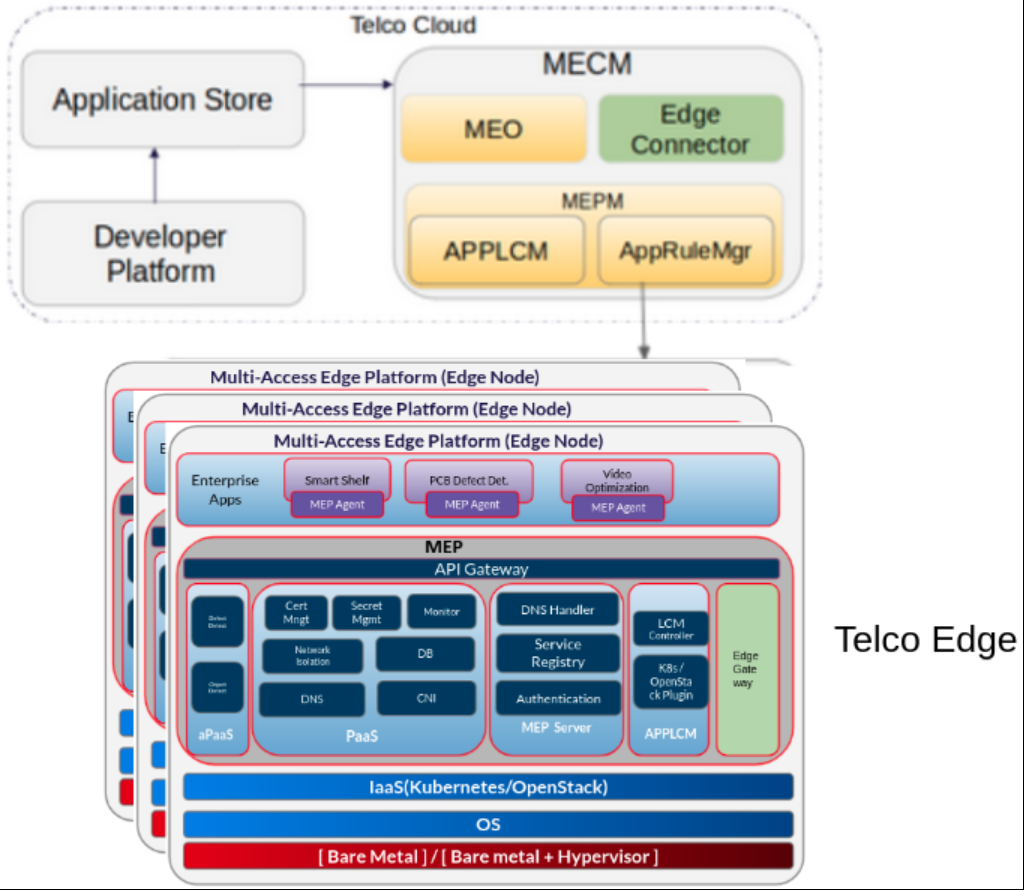
\includegraphics[width=13cm]{./images/akraino-ealtedge.png} % CHANGE THIS FIGURE
	\caption{My PNG image}
\end{figure}

The deployment of EALTEdge is quite flexible, allowing to deploy everything as containers in one node (bare metal or virtual) or it can be deployed in multiple, typically two nodes. Furthermore, the deployment is managed through provided ansible playbooks to simplify the whole process. 

Because EALTEdge provides a general MEC system, which closely follows ETSI MEC specifications and also offers a development environment for MEC apps, it seems like an ideal platform for the testbed development. However, upon testing in lab environment, it was discovered that EdgeGallery servers forbid requests of downloading the tarballs containing the software. Therefore, while EALTEdge or even EdgeGallery alone seem like very promising projects, they could not be leveraged in testbed development.

\section{Intel Edge Projects}
Beside the Akraino project, another primary mover within edge software development is Intel. Intel develops commercial end-to-end edge solutions for their customers, but they also offer open-source variants for developers to prototype on. The range of edge-oriented products currently offered by Intel and the licenses under which they are released are shown in Figure 12. A successful open-source solution by Intel was Open Network Edge Services Software (OpenNESS), which at some point gained a lot of momentum within MEC open-source community, it is heavily reference in [d] and moreover, several Akraino blueprints reference OpeNESS as a platform they were initially built on [r, u]. However, the OpeNESS project was shut down and transitioned towards Smart Edge Open. Both platforms will be introduced in the following two subsections.
\begin{figure}[ht]
	\centering
	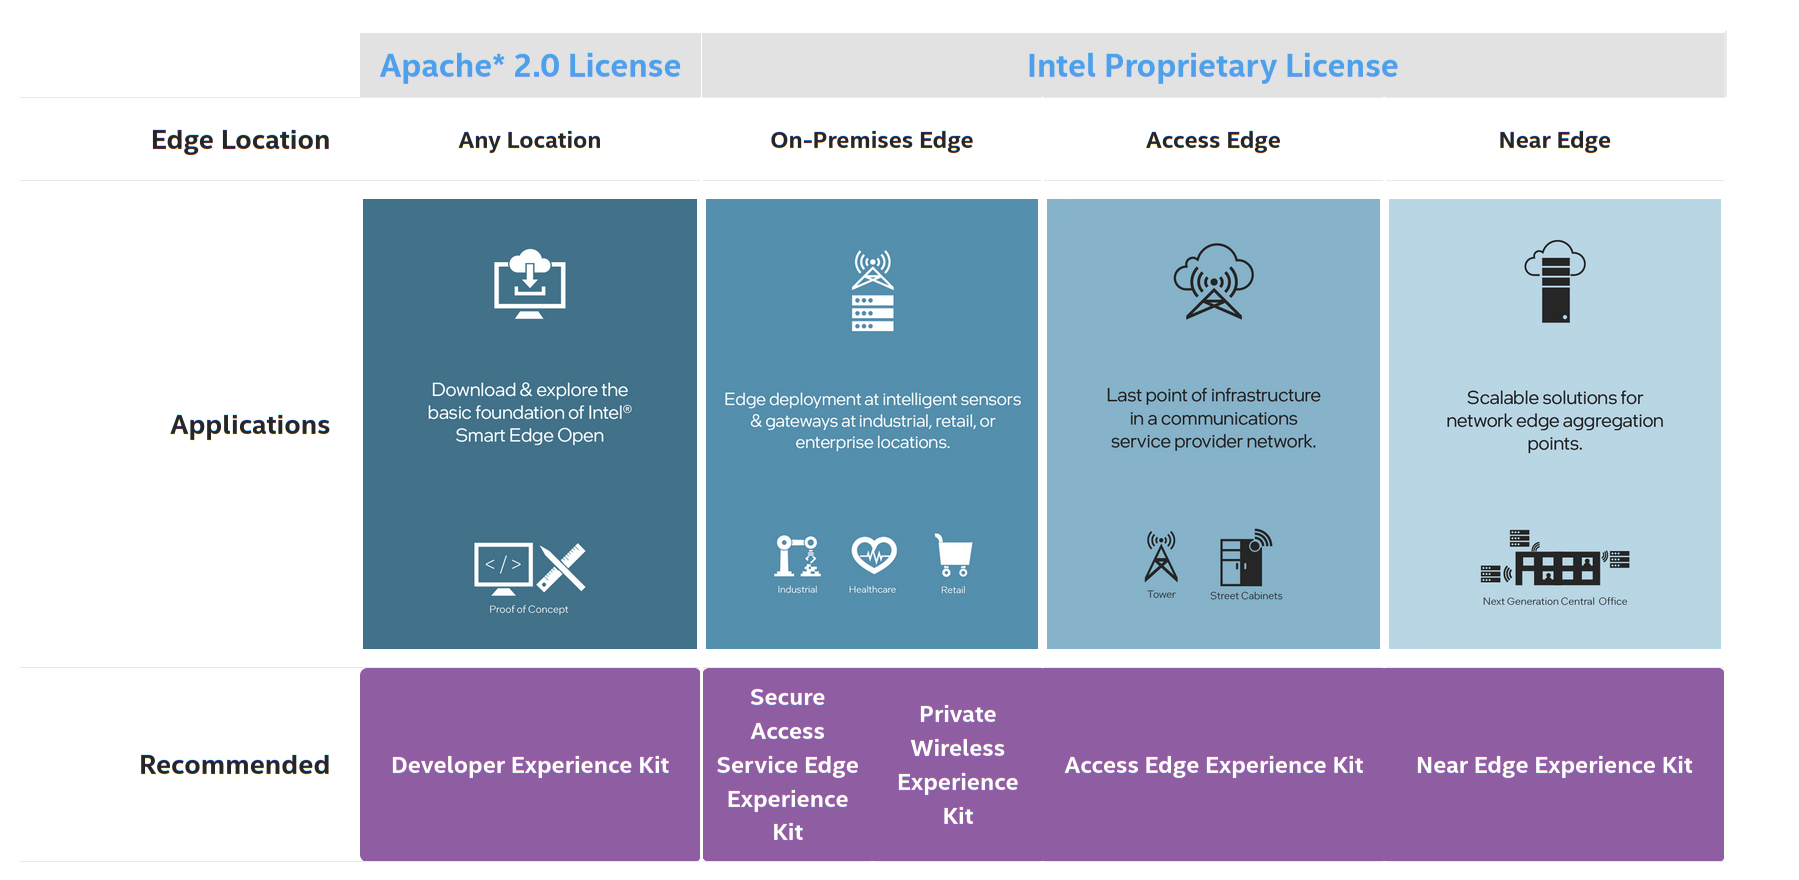
\includegraphics[width=13cm]{./images/intel-solu.png} 
	\caption{My PNG image}
\end{figure}

\subsection{OpenNESS}
OpenNESS is a software toolkit that enables building custom platforms for edge computing use cases, including MEC, capable of onboarding and managing applications. Although OpenNESS did not strictly follow the ETSI MEC specifications, it was inspired by them and also references 3GPP and O-RAN specifications that were used to develop APIs for integration with 5G mobile networks [d]. It should be noted that Intel offered its own solution for 5G CN emulation, which was probably compatible with OpenNESS, though that was not part of the open-source package and was offered as a commercial product. [v] 

OpenNESS was built on top of Kubernetes and highly optimized for edge computing. A typical deployment consists of an OpenNESS Kubernetes Edge Node and an OpenNESS Kubernetes Control plane, as shown in Figure 13. [v]
\begin{figure}[ht]
	\centering
	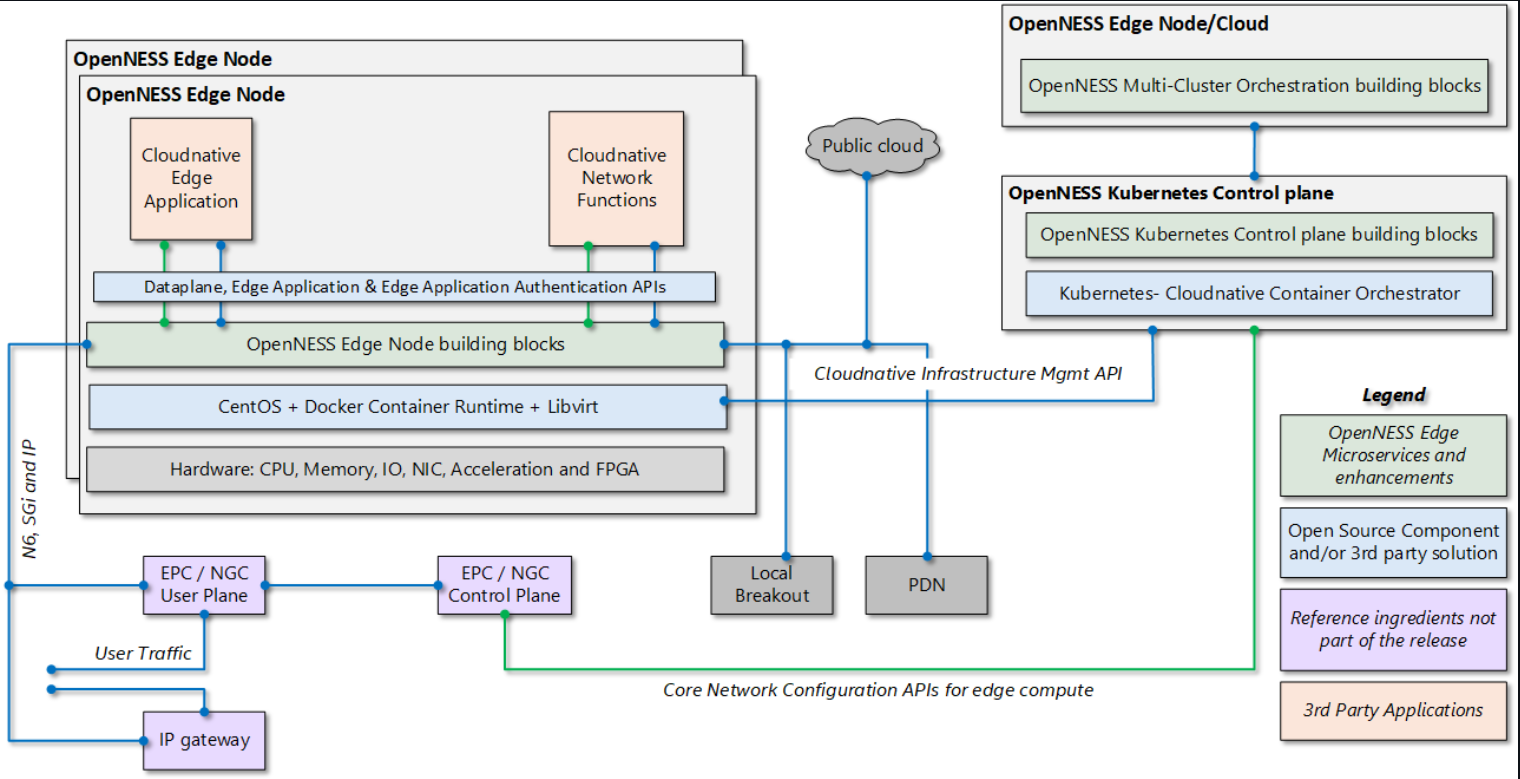
\includegraphics[width=13cm]{./images/openness.png} 
	\caption{My PNG image}
\end{figure}

\subsection{Smart Edge Open}
Smart Edge Open (SEO) is a result of Intel’s efforts to unify development of its open-source and commercial products. SEO follows the basics of OpenNESS architecture, as it is also built on top of Kubernetes and the basic deployment model consists of a control node and an edge node. [w] The resulting architecture is shown in Figure 14. Even though SEO development initially started as a rebranding of OpenNESS, the documentation of SEO is not as rich and it further distances itself from the ETSI MEC architecture. Eventually, while the transition from OpenNESS to SEO may have improved the platform’s integration into Intel ecosystem, it distances itself from open-source MEC community, where strict following of standardized architecture is necessary to ensure interoperability between individual projects. 

Even though it was argued that due to its distancing from strict ETSI MEC reference architecture, SEO is not an optimal solution for testbed development, it was still tested in our lab environment. However, the deployment of the platform was unsuccessful. SEO uses Intel’s own provisioning software and while it should simplify the deployment, it makes the process of troubleshooting unfeasible, when an issue is encountered.
\begin{figure}[ht]
	\centering
	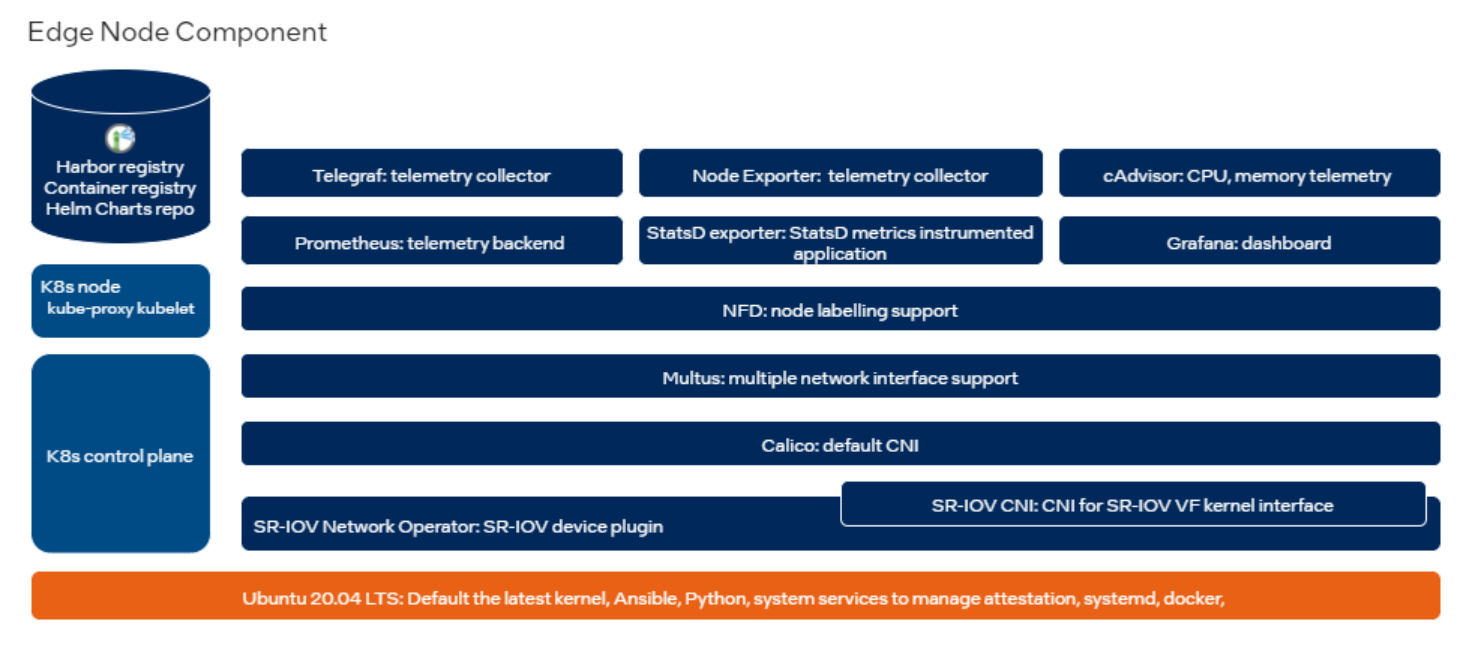
\includegraphics[width=13cm]{./images/intel-seo.png} 
	\caption{My PNG image}
\end{figure}

\section{EURECOM and OpenAirInterface Projects}
The two following projects have been developed by EURECOM and are closely related to OpenAirInterface (OAI), the mobile network emulation platform that is now maintained by OAI Software Alliance (OSA). EURECOM though continues to be involved in the development OAI and plays a key role in expanding the scope of OAI to network slicing or MEC.
\subsection{LL-MEC}
Low latency MEC (LL-MEC) was introduced in 2018 as the first open-source low latency MEC platform, enabling mobile network monitoring, control and programmability [y]. While it was developed in compliance with 3GPP and ETSI specifications, these specifications are not related to 5G MEC integration referenced in chapter 2, since LL-MEC was developed as a 4G MEC solution. One possible deployment of LL-MEC is shown in Figure 15, which also demonstrates that LL-MEC uses Open vSwitch for user plane. Since this thesis puts main focus on integrating MEC in 5G mobile networks, the LL-MEC has not been chosen as the platform for testbed development.
\begin{figure}[ht]
	\centering
	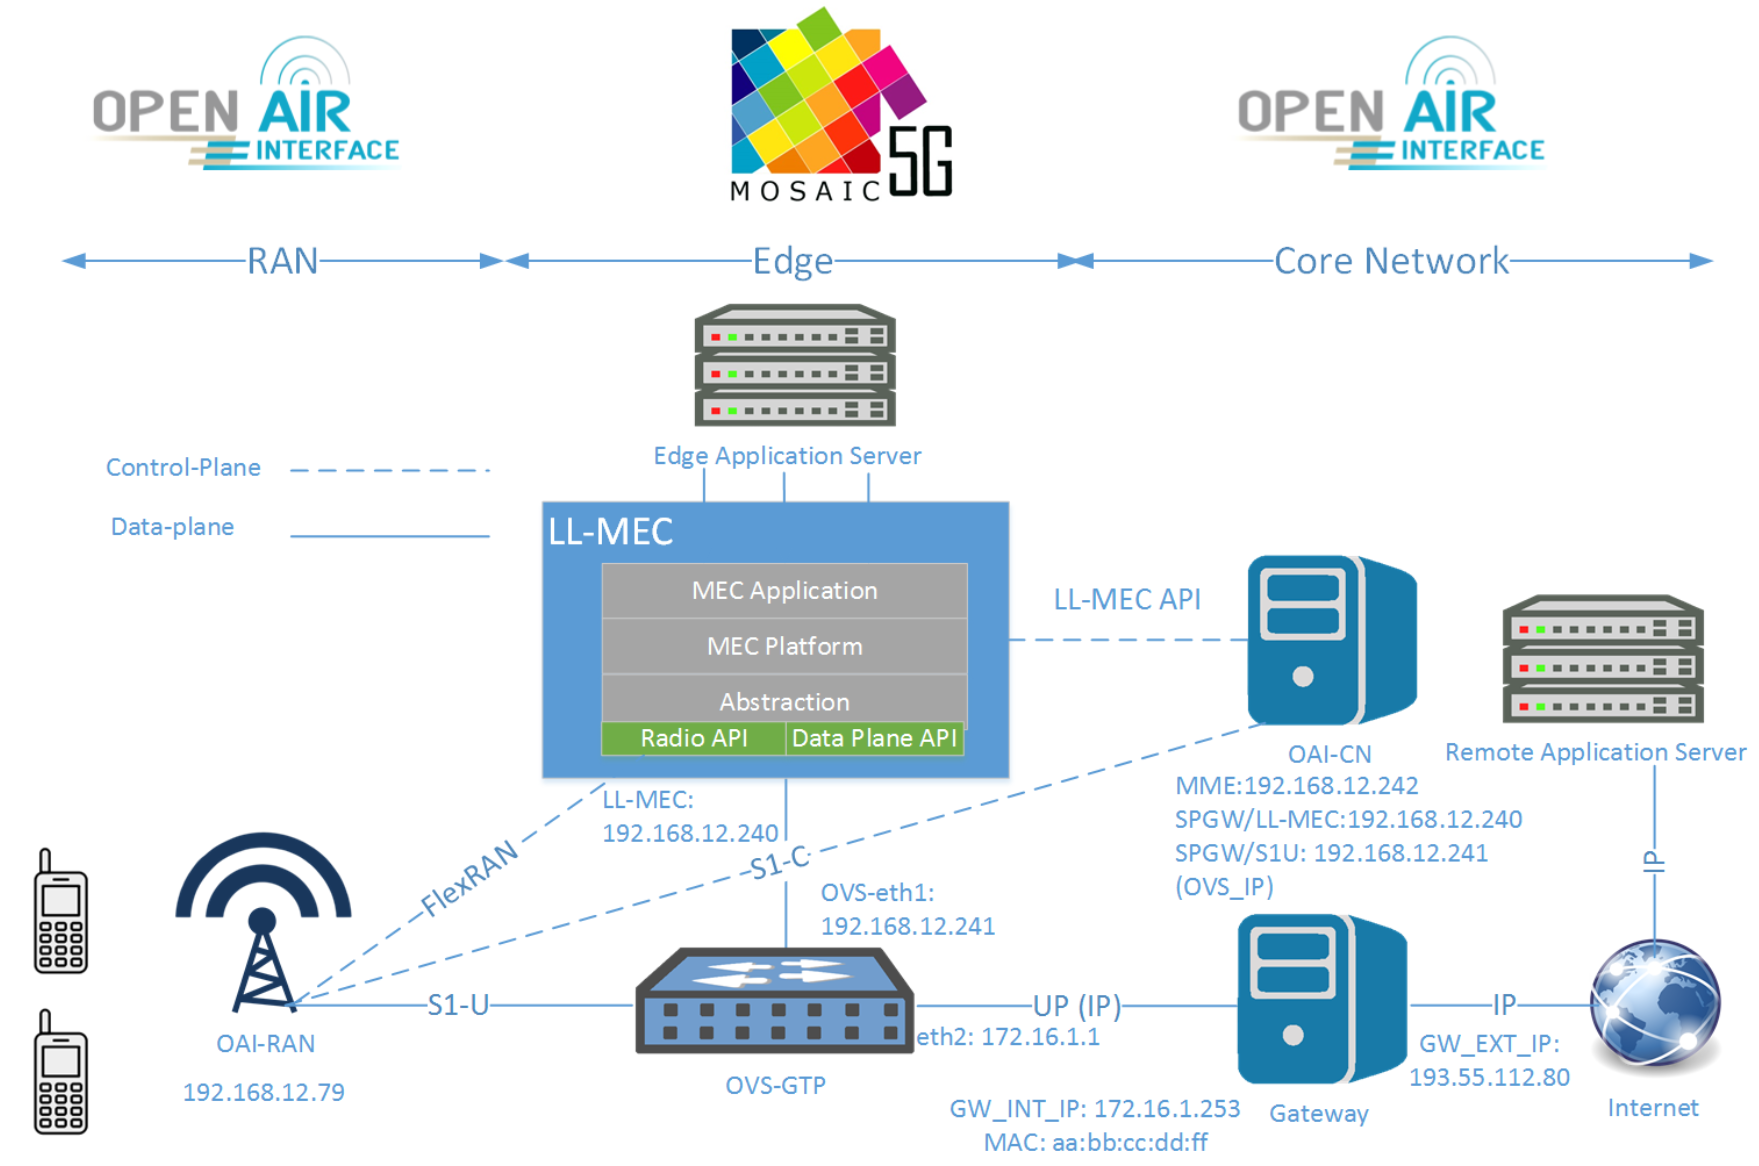
\includegraphics[width=13cm]{./images/ll-mec.png} 
	\caption{My PNG image}
\end{figure}

\subsection{MEC platform by EURECOM}
This MEC Platform (MEP) has been only recently developed by EURECOM and is closely integrated with OAI emulated 5G network. At the time of writing, the MEP is very much a work in progress as it only implements a MEP environment for registry and discovery of MEC services and offers its own implementation of Radio Network Information Service (RNIS) [x]. However, it has several traits that make it a very viable candidate for VEC testbed development. Its integration with the OAI would significantly reduce the integration implementation overhead. Moreover, it promises to follow ETSI MEC as well as O-RAN specifications. And finally, the developers have already outlined that it is intended to implement traffic rules control via communicating with PCF in 5G CN. This would mean that the project is aiming for a MEC implementation very close to the standardized approach extensively described in chapter 2. The components thus far developed are shown in Figure 16.
\begin{figure}[ht]
	\centering
	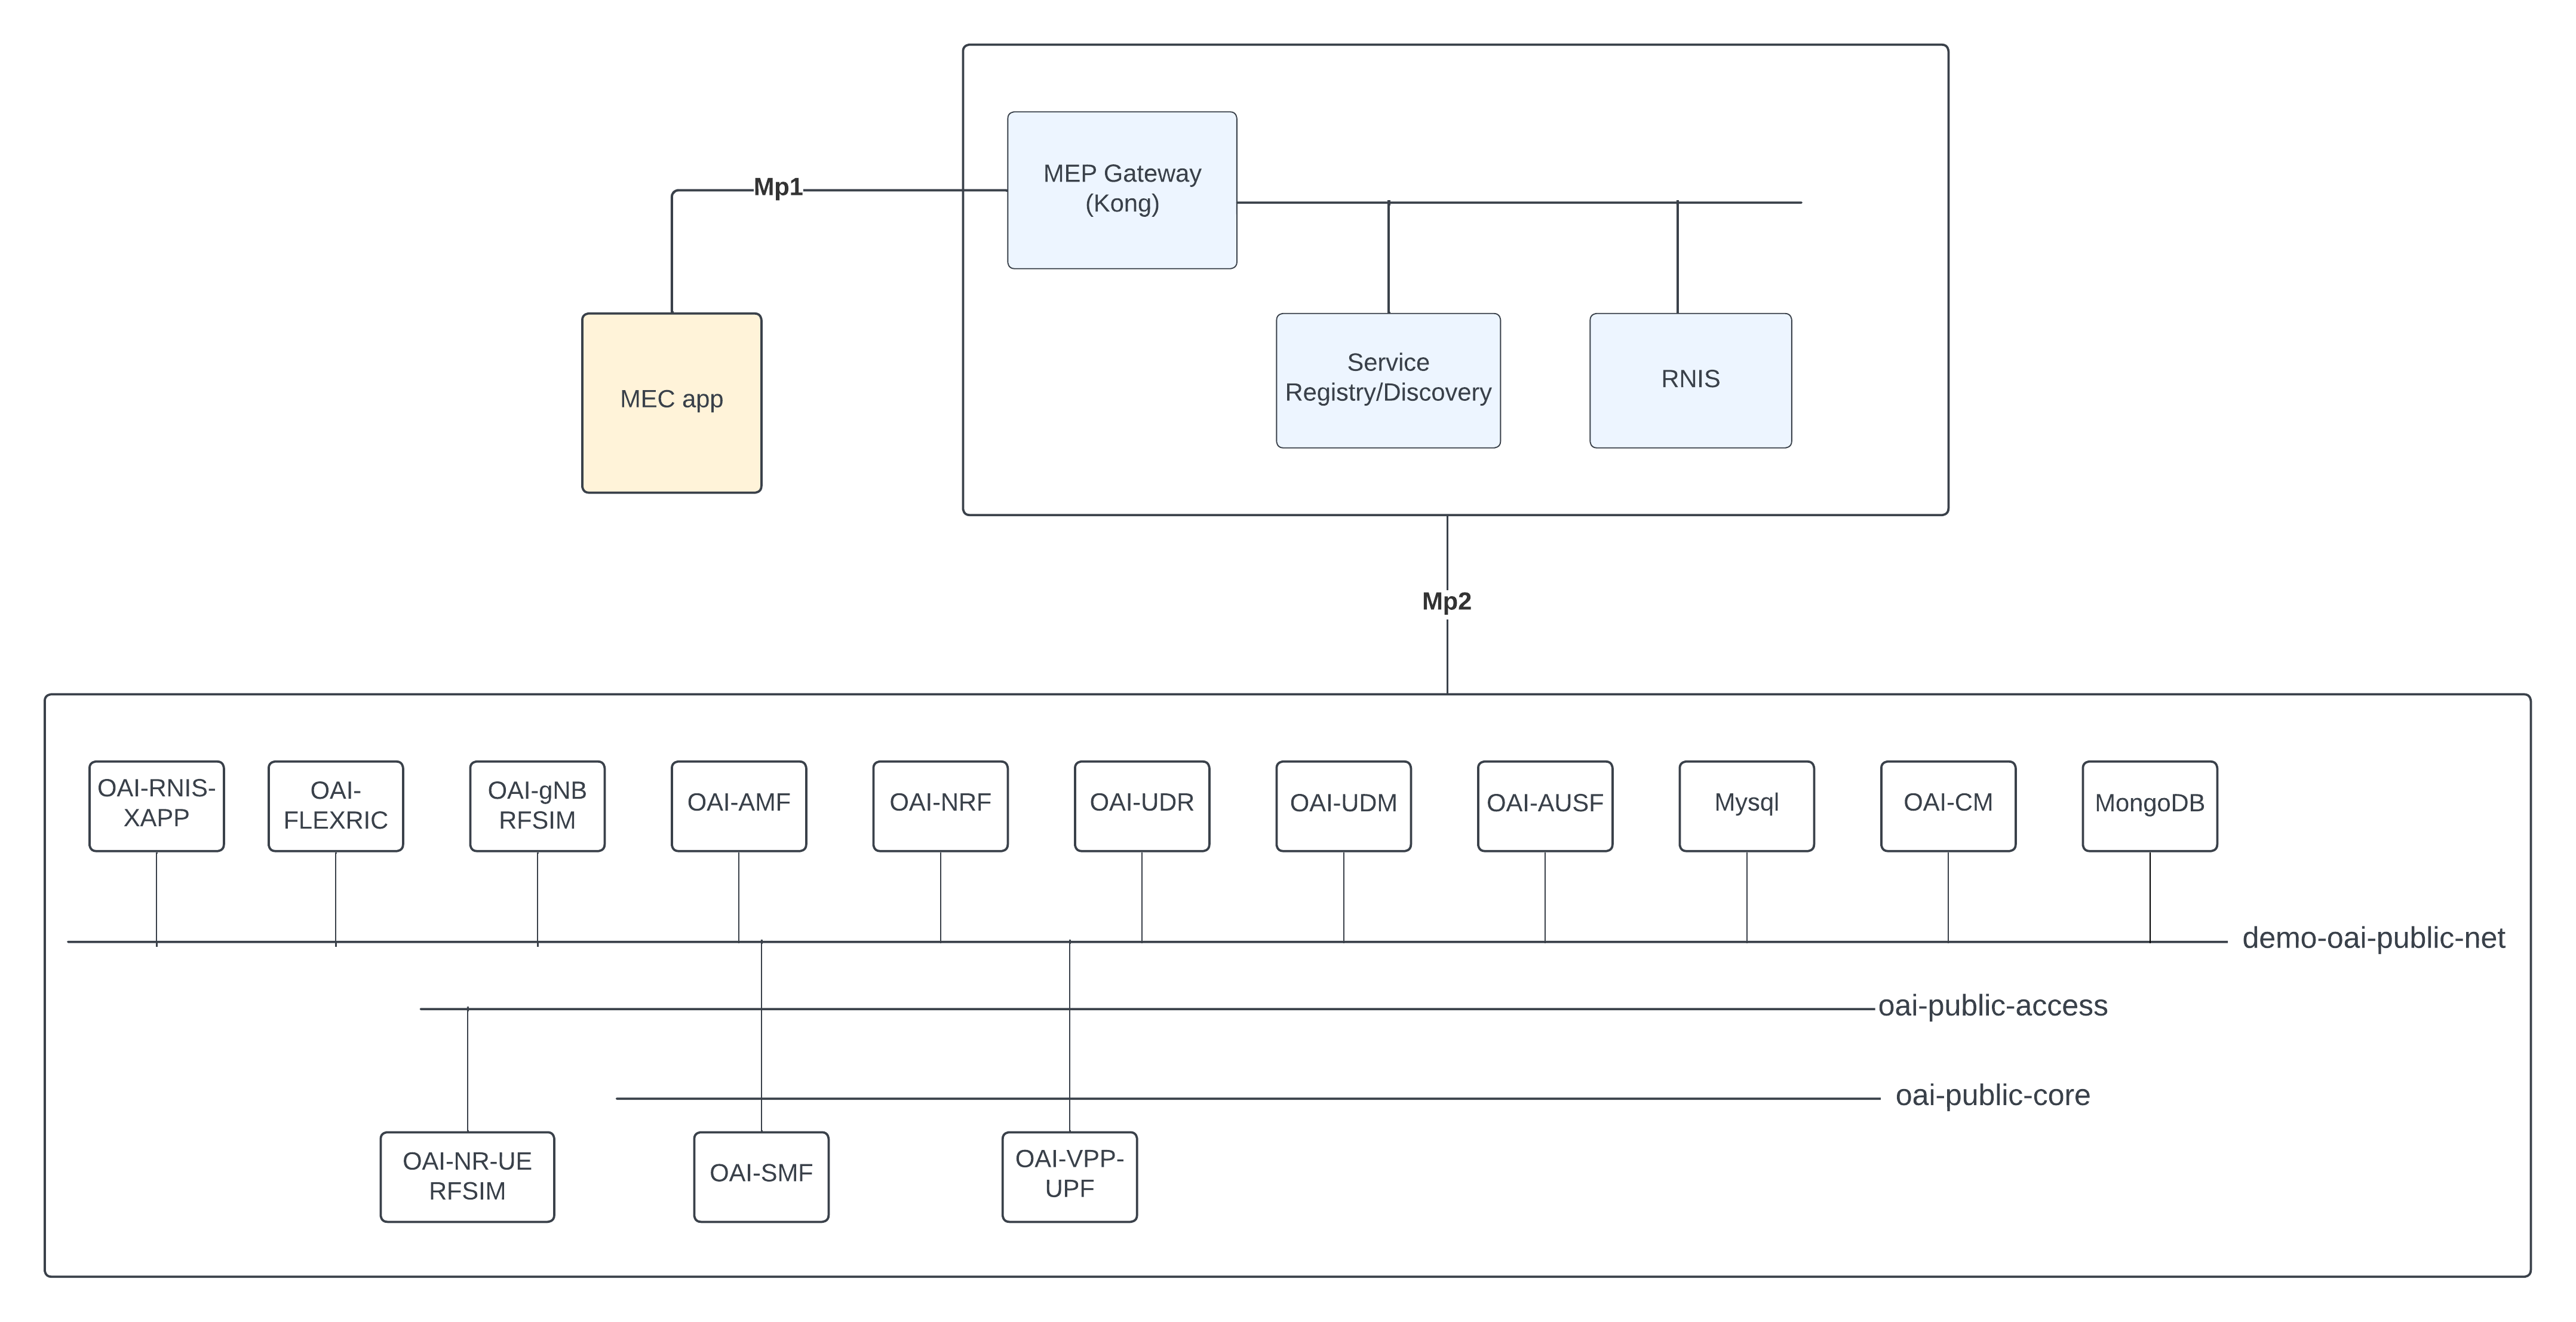
\includegraphics[width=13cm]{./images/OAI-MEP.png}
	\caption{My PNG image}
\end{figure}

\section{Other MEC projects}
\subsection{AdvantEDGE}
AdvantEDGE is a mobile edge emulation platform running on Docker and Kubernetes. Its main ambition is to help MEC app developers decide where in the network edge their application should run and how different network characteristics such as latency, packet loss or jitter impact their application’s QoS. This is achieved through emulation of mobile network with the possibility to test the application with different network characteristics settings and different deployment models (how close to the user the app is run). On top of that, the platform enables triggering of mobility events and application relocation even for stateful applications. The platform is not intended to emulate any part of the ETSI MEC reference architecture, but it implements various ETSI MEC APIs, such as RNIS, Location Service or App Enablement Service. The high-level overview of AdvantEDGE micro-service based architecture is shown in Figure 17.
\begin{figure}[ht]
	\centering
	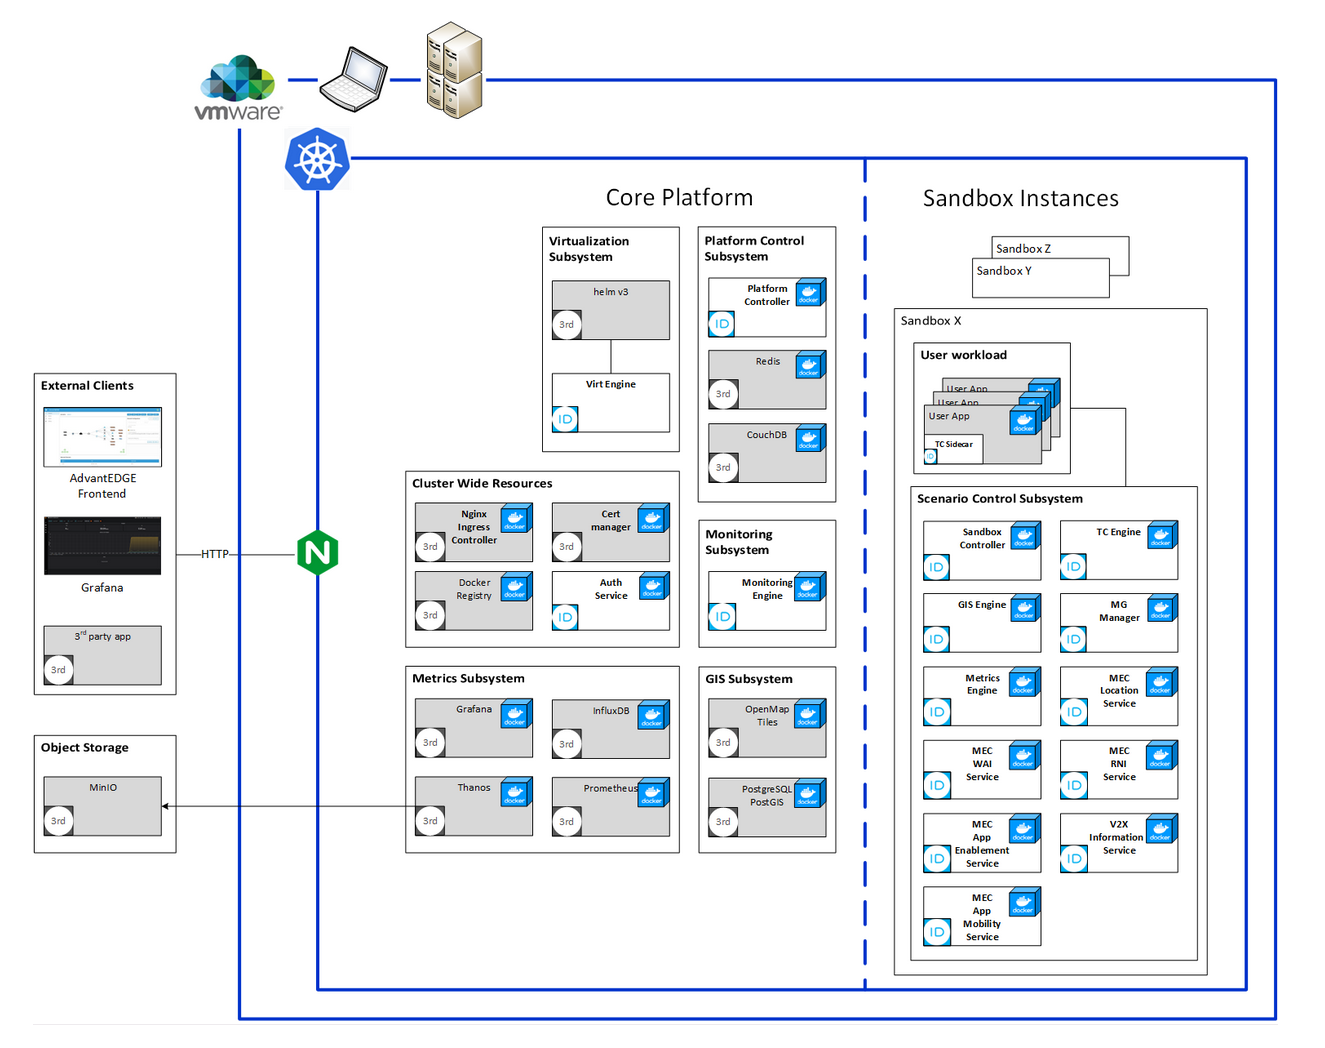
\includegraphics[width=13cm]{./images/advatnedge.png} 
	\caption{My PNG image}
\end{figure}

AdvantEDGE was successfully deployed in our lab setup, however, it was deemed not suitable for the purposes of the testbed development, which puts a strong emphasis on the platform architecture and the underlying mobile network.

\chapter{Mobile network emulation: \texorpdfstring{\\ \mbox{OpenAirInterface}}{OpenAirInterface}}
The goal of this chapter is to provide an overview of an open-source mobile network emulation platform OpenAirInterface (OAI). OAI has the ambition to democratize the research and development of wireless access technologies through delivering a 3GPP compliant software stack for both RAN and CN. The OAI software offers different levels of mobile networks simulation or emulation in flexible deployment scenarios and is intended to run on general purpose hardware [z]. OAI was originally founded by EURECOM, and its development is overseen by OSA, which has the goal of promoting the adoption of OAI across both academia and industry. 

OAI development is split into different projects. The two biggest ones are focused on developing the solutions for RAN and CN. While those are definitely the core of OAI, its focus spans further and exploits smart solutions regarding mobile networks’ orchestration and programmability under Mosaic5G project. The following sections offer a brief introduction to all of these projects and discuss how they are going to be leveraged in OAI based VEC testbed.

\section{OAI RAN}
OAI RAN offers modems for the UE and base station (eNB in 4G and gNB in 5G). These modems are developed with respect to 3GPP specifications and therefore, OAI RAN implements the entire 5G New Radio (5G-NR) protocol stack [aa]. This thesis is focused primarily on the CN architecture, therefore, the individual protocols of 5G NR will not be exploited in great detail. Below is an example of 5G NR user plane protocol stack with brief introduction of individual layers based on [a].

\begin{figure}[ht]
	\centering
	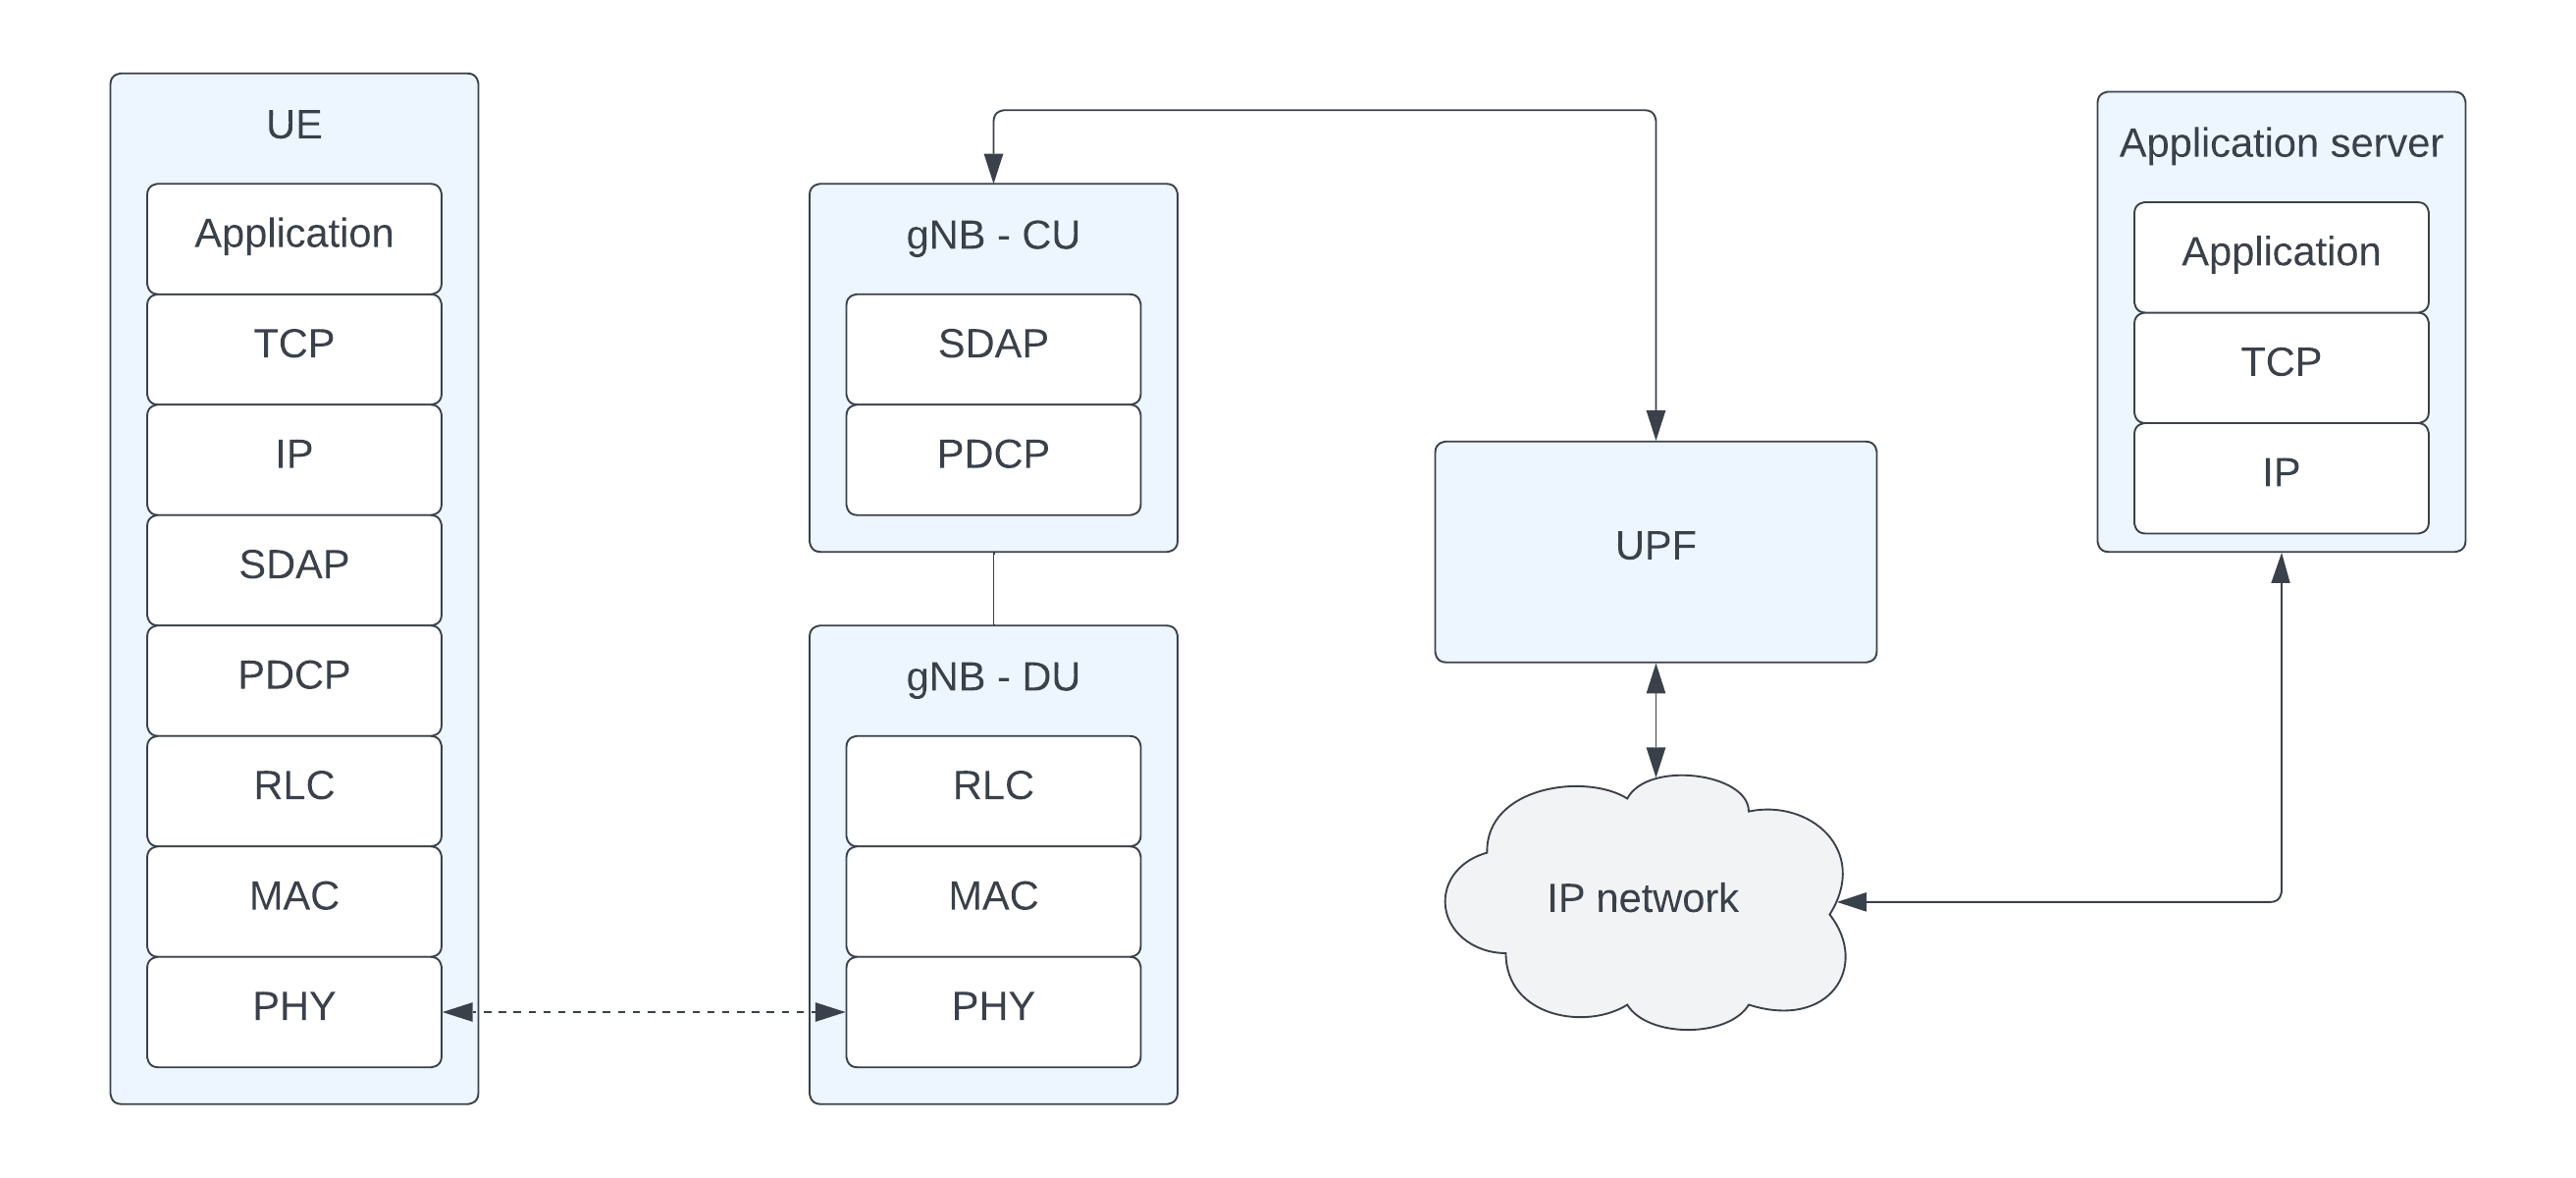
\includegraphics[width=13cm]{./images/5G-NR-protstack.png} 
	\caption{My PNG image}
\end{figure}
The three topmost layers are the application layer, the Transmission Control Protocol (TCP) and Internet Protocol (IP). This is common for any IP-based network, including 4G and 5G mobile networks.

The 5G NR user plane protocol stack:
\begin{itemize}
	\item Service Data Application Protocol (SDAP): responsible for mapping of QoS bearers to radio bearers, new layer in NR.
	\item Packet Data Convergence Protocol (PDCP): performs IP header compression, ciphering and integrity protection.
	\item Radio Link Control (RLC): segmentation and retransmission handling.
	\item Medium Access Control (MAC): multiplexing of logical channels, hybrid retransmission and scheduling.
	\item Physical Layer (PHY): coding and decoding, modulation and demodulation or multi-antenna mapping.
\end{itemize}
In control plane, the lower-level protocols are the same, but on top of PDCP there is RRC and NAS.
\begin{itemize}
	\item Radio Resource Control (RRC): setup and release of radio bearers, mobility management, CP signaling.
	\item Non-Access Stratum (NAS): signaling messages between UE and CN for management of UE mobility and network selection.
\end{itemize}
For a better understanding of current OAI 5G NR capabilities, some general features based on [aa] are listed below:
% ---------------------
% add a table with basic features for OAI NR
% ---------------------
OAI is designed to serve as a development tool for accurate mobile networks simulations and emulations. For this purpose, OAI enables different simulation models: RFsimulator, L2 nFAPI simulator and running with true radio heads. RFsimulator replaces the radio heads and allows connecting the UE to eNB or gNB via network interfaces. It is the optimal model to start testing OAI as it significantly decreases the deployment overhead. L2 nFAPI simulator allows connecting the UEs and eNB or gNB via nFAPI (Network Functional API), thus shortcutting the PHY layer. Finally, OAI is designed to operate with true radio interface, using Customer-Off-The-Shelf (COTS) hardware, such as USRP (Universal Software Radio Peripheral) for the e/gNB and regular COTS UE. [aa] 

The development of OAI 5G CN is an ongoing process, while evolution from LTE in 4G to NR in 5G seems to be complete with OAI enabling standalone 5G deployment, OSA defined the short-term goals of OAI as performance improvement or integration with smart RAN solutions developed within the Mosaic5G group. [dd]
\section{OAI CN}
OAI 5G CN project group develops open-source solution for standalone 3GPP compliant 5G CN that is capable of enabling various 5G use cases. The 5G CN components are continuously tested with open-source as well as commercial RAN solutions [bb]. The OAI 5G CN has been gradually developed from 4G EPC to the 5G CN architecture, extensively described in chapter 2. In fact, this work is still ongoing, with the current state-of-the-art shown in Figure 21.
\begin{figure}[ht]
	\centering
	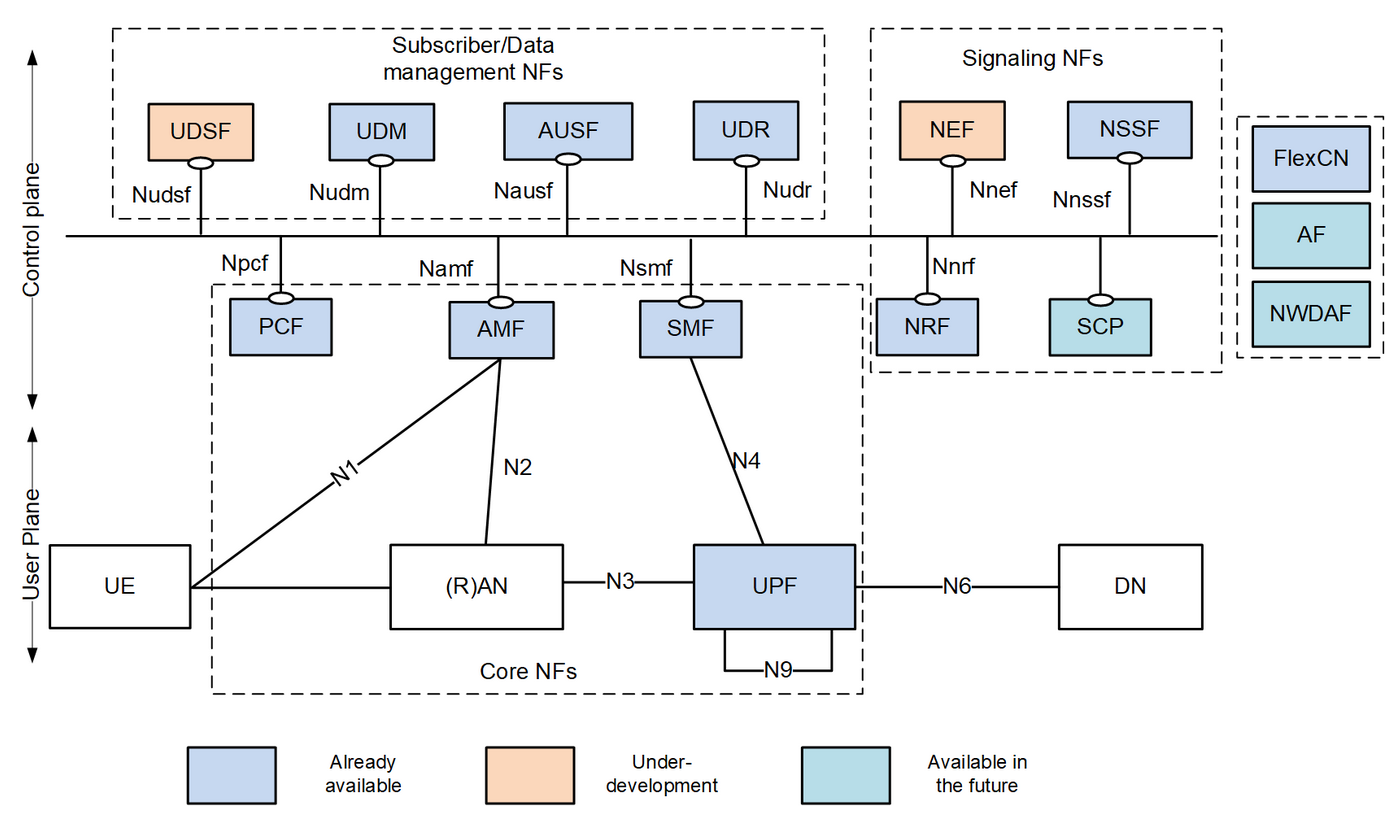
\includegraphics[width=13cm]{./images/OAI-CN-soa.png} 
	\caption{My PNG image}
\end{figure}
According to [bb], OAI 5G CN currently supports many of the key workflows described in chapter 2, such as UE connection, registration and session management. Network slicing is already partially supported, but a key interface for opening the CN to third parties, the AF, is not yet available. This is important from the perspective of integrating an open-source MEC system solution with OAI CN because AF should play a key role in providing the means of accessing the CN’s SBA for MEC orchestrator or MEC platform. 

The flexibility of OAI 5G CN design allows for different deployment models based on deployed NFs. In the minimalist example supporting basic session management procedures, AMF, SMF, NRF and UPF comprise the whole CN. The basic deployment model consists of the minimalist model and AUSF, UDM and UDR [bb]. UDR (Unified Data Repository) was not described in chapter 2, it is a NF providing storage and retrieval of structured data for PCF, NEF and UDM [ee]. Finally, slicing deployment model utilizes the basic model with NSSF [bb]. 

As was the case with OAI 5G RAN project, OAI 5G CN is still being developed to offer new capabilities and enable new use cases. During 2022, OAI released PCF and currently works on integrating PCF induced traffic steering. This is a key part of the MEC integration described in chapter 2.
\section{Mosaic5G}
Mosaic5G is a project group within OAI focused on transforming the underlying OAI RAN and CN into agile platforms providing ecosystem for use cases ranging from centralized network control to edge deployments [dd]. The primary focus of Mosaic5G project group can be dissected into four main projects as defined in [dd]:
\begin{itemize}
	\item The O-RAN E2 protocol – E2 agent
	\item A Flexible RAN Intelligent Controller (FlexRIC)
	\item A Flexible Core Controler (FlexCN)
	\item Higher layer RAN and CN operator – Tirematics
\end{itemize}
Currently, most of the Mosaic5G project group’s work is centered around FlexRIC and its integration with the rest of the OAI software [dd]. In fact, the OAI MEP discussed in previous chapter also utilizes FlexRIC as a key component [x]. 
\chapter{VEC testbed}
The final chapter describes the implementation of testbed for VEC as the primary goal of the thesis. The structure of the following text is as follows: below, the whole task is dissected into three key stages, then each stage is examined in individual subsequent sections.
\begin{itemize}
	\item[\textbf{Stage 1:}] VEC testbed design leveraging chosen open-source projects 
	\item[\textbf{Stage 2:}] creating a blueprint for future VEC applications development
	\item[\textbf{Stage 3:}]  evaluation of set up testbed against cloud deployment
\end{itemize}

\section{VEC testbed design}
The final testbed design leverages the OAI MEP, introduced in chapter \ref{ch:o-sMEC}. While there, the focus was primarily on evaluating it against other MEC projects in terms of network architecture, this section describes the individual components from developer’s perspective. OAI MEP does not comprise the whole MEC system, but it provides an ETSI compliant MEP with a service-based environment, fully compatible with the underlying OAI RAN and CN. Such setup is sufficient for experimentation with VEC applications, such as task offloading. 

The leveraged platform is a blueprint showcasing OAI MEP with RNIS and it integrates five key projects as shown in Figure 22 [gg]:
\begin{itemize}
	\item OAI 5G RAN
	\item OAI 5G CN
	\item OAI MEP
	\item OAI Configuration Manager (CM)
	\item RNIS
\end{itemize}
\begin{figure}[ht]
	\centering
	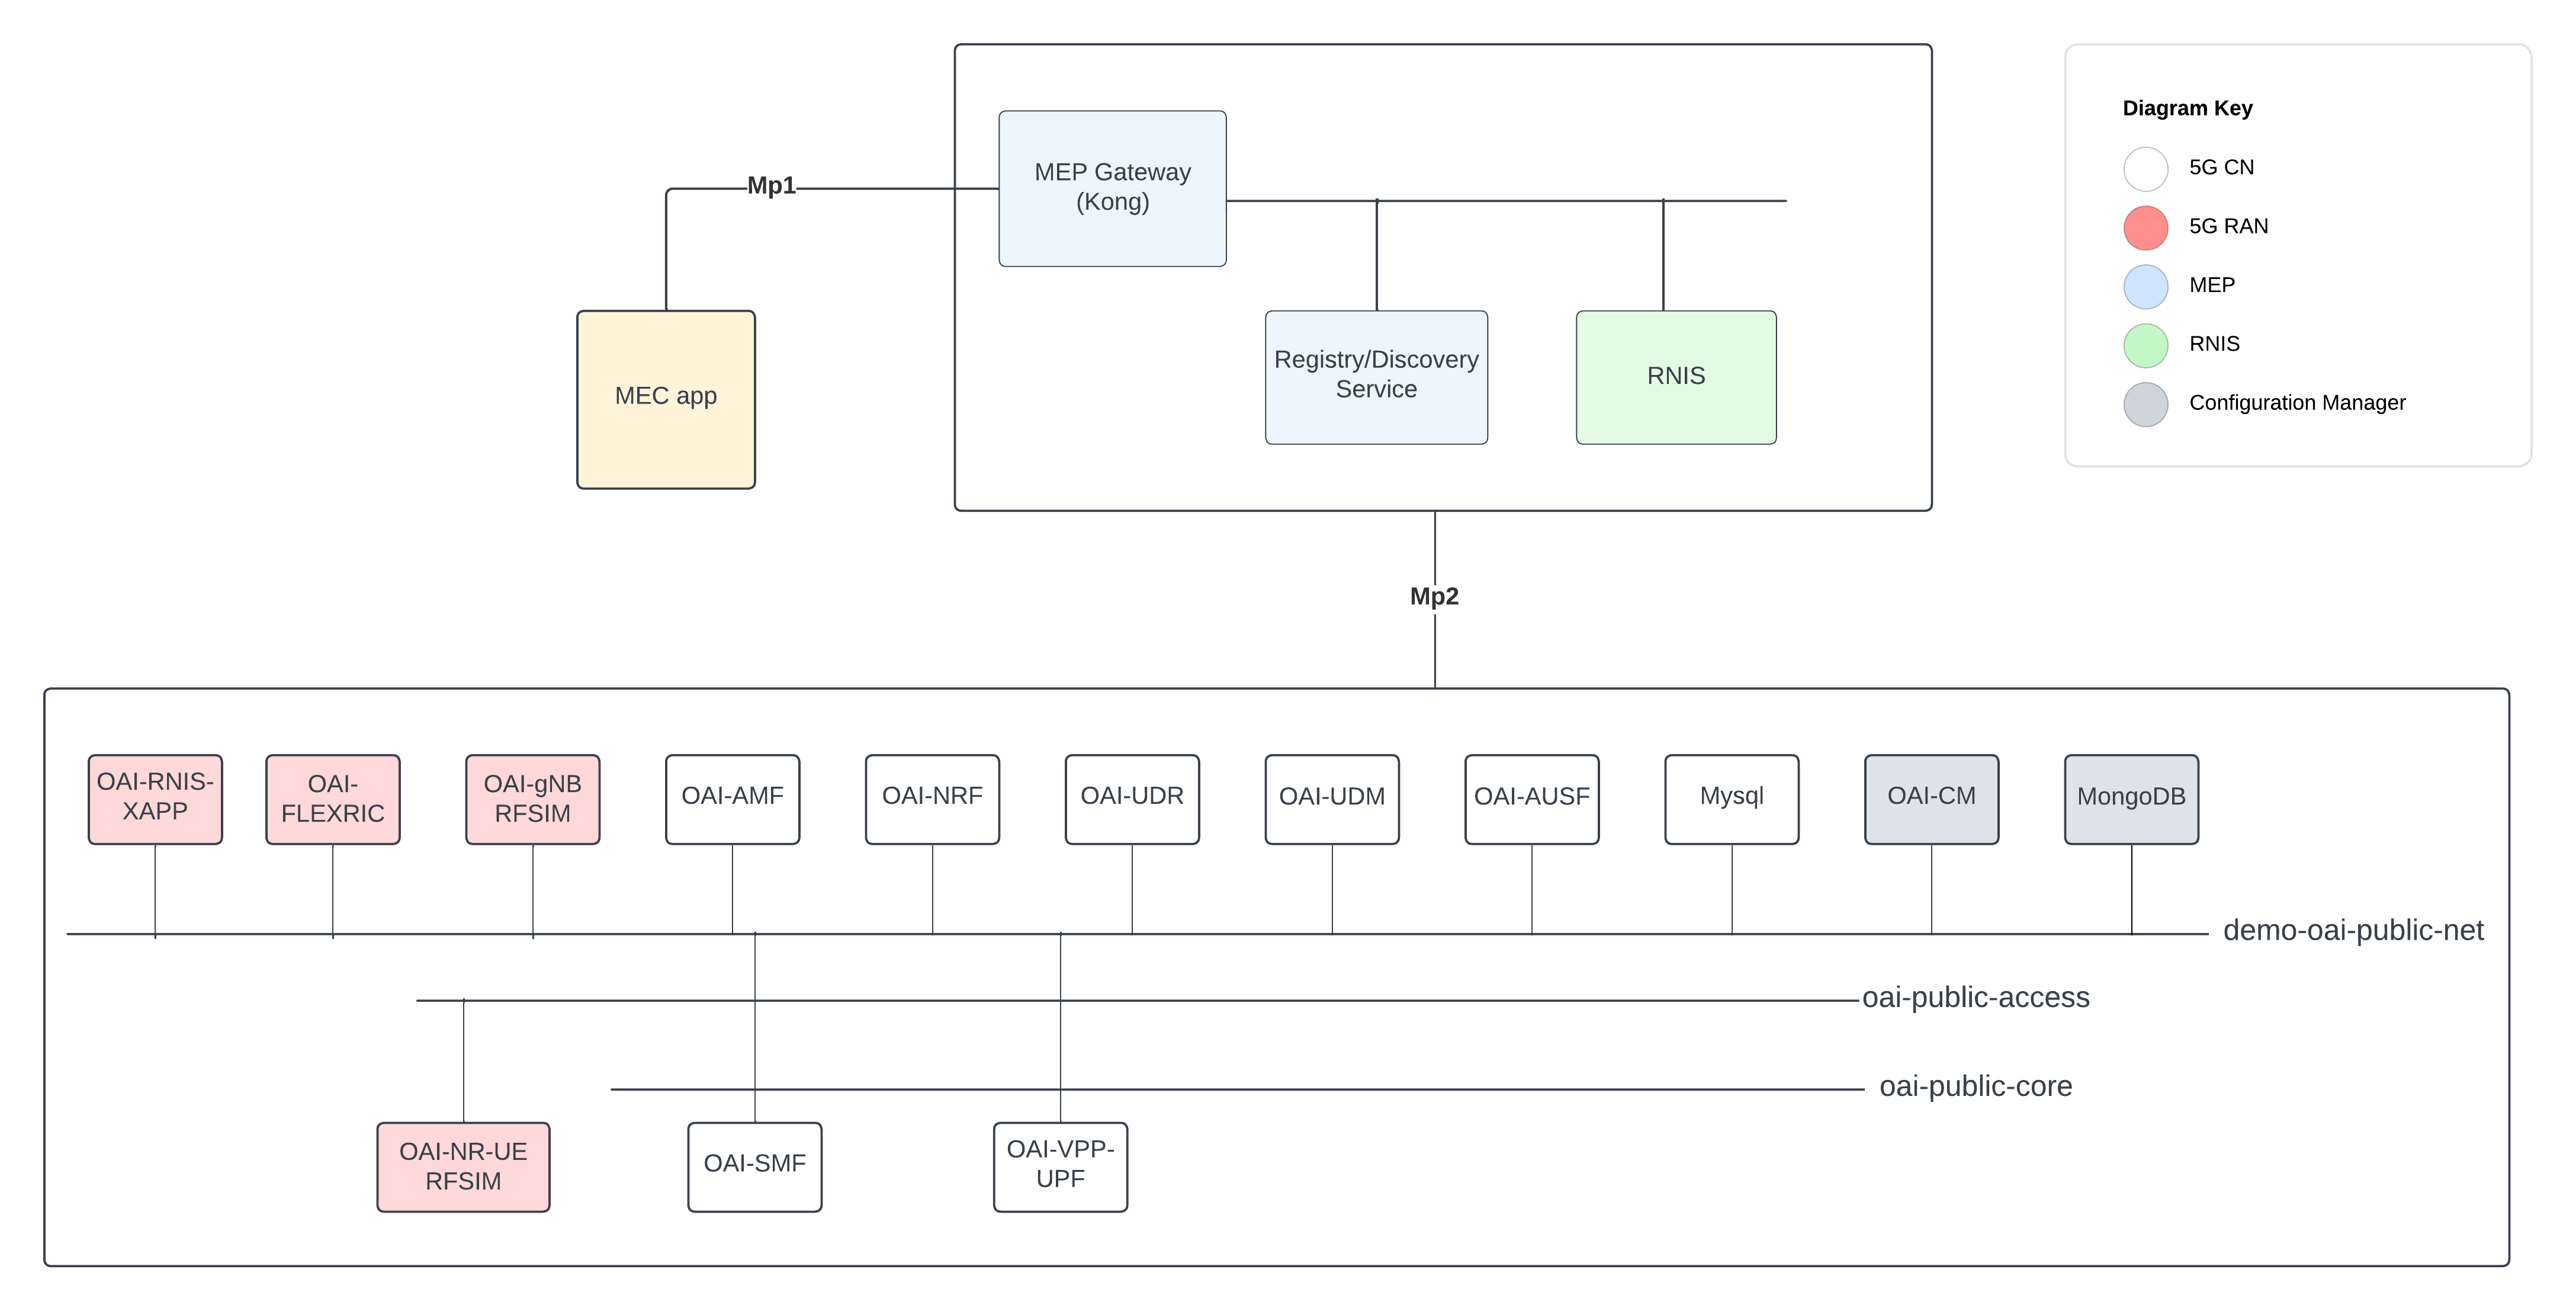
\includegraphics[width=13cm]{./images/OAI-MEP-parts.png} 
	\caption{My PNG image}
\end{figure}
This blueprint showcases how MEC apps can consume services, such as RNIS, via the Mp1 interface [gg]. For RNIS to be able to consume mobile network Key Performance Indicators (KPIs) via Mp2 and then expose them via Mp1 to MEC apps, the OAI mobile network required new features to be implemented. The OAI 5G CN is run in a basic deployment, as shown in Figure 22, but the RAN leverages an O-RAN xApp and Mosaic5G FlexRIC on top of the modules for UE and gNB. The xApp provides a northbound interface for the RNIS to subscribe to radio related KPIs [ff]. The OAI configuration manager then provides the functionality to subscribe to AMF and SMF events [hh]. 

A key component of the OAI MEP is the MEP Gateway, which acts as a reverse proxy, routing the Mp1 traffic to the right service [x]. The reverse proxy is implemented leveraging Kong. It hides the underlying service nodes from the clients and routes client’s requests to the right service nodes. This means that all registered services can be accessed via the MEP Gateway. 

The Discovery and Registry Service has the responsibility of exposing REST API for the Mp1 interface allowing the MEC apps to do the following, based on [x]:
\begin{itemize}
	\item Discover existing services (GET)
	\item Filter hosted MEC services based on service type (GET)
	\item Register a new service (POST)
	\item Delete a hosted MEC service (DELETE)
\end{itemize}
The OAI MEP blueprint delivers docker-compose scripts for the deployment of all the containers. Furthermore, the basic deployment uses rfsim, although [gg] claims that it is possible to run with USRP radio heads and that it was tested in their lab. 

After a successful deployment, it should be possible to ping the internet from the UE container via its \verb |oaitun_ue1| interface. In our setup, it looks like this:
\begin{verbatim}
	root@9929963b00c2:/opt/oai-nr-ue# ping -c 3 -I oaitun_ue1 comtel.fel.cvut.cz
	PING glumhosting.fel.cvut.cz (147.32.210.146) from 12.1.1.2 oaitun_ue1:\
	56(84) bytes of data.
	64 bytes from glum-146.feld.cvut.cz (147.32.210.146):\
	icmp_seq=1 ttl=59 time=8.64 ms
	64 bytes from glum-146.feld.cvut.cz (147.32.210.146):\
	icmp_seq=2 ttl=59 time=5.43 ms
	64 bytes from glum-146.feld.cvut.cz (147.32.210.146):\
	icmp_seq=3 ttl=59 time=5.06 ms

	--- glumhosting.fel.cvut.cz ping statistics ---
	3 packets transmitted, 3 received, 0% packet loss, time 2003ms
	rtt min/avg/max/mdev = 5.062/6.382/8.649/1.610 ms
\end{verbatim}

To verify that the RNIS works properly, it should be possible to access its service with the HTTP GET method from the Command Line Interface (CLI). This is the result achieved in our setup:
\begin{verbatim}
	lab@lab-HP-Z4-G4-7-Workstation:~/blueprints/mep/examples$ curl -X 'GET'\
	'http://oai-mep.org/rnis/v2/queries/layer2_meas' -H 'accept: application/json'
	[
	{
		"KPIs": {
		"bler_dl": {
			"kpi": "bler_dl",
			"labels": {
			"amf_ue_ngap_id": 1
			},
			"source": "RAN",
			"timestamp": 1683903896587163,
			"unit": null,
			"value": 5.605193857299268e-45
	...
\end{verbatim}

\section{VEC application blueprint}
This stage is split into two subsections, with the first one covering the service registration and the second one demonstrating implementation of a MEC app consuming services offered by the OAI MEP.
\subsection{Service registration}
The registration and discovery service of OAI MEP can be accessed via its Graphical User Interface (GUI) on the host 192.168.70.5 or via the MEP Gateway: \\ \verb |http://oai-mep.org/service_registry/v1/ui|. It should be noted that for the latter to work, the oai-mep.org domain needs to be added to the local machine DNS, which is documented in [gg]. The GUI offers the services mentioned in the previous section. After a successful deployment, the discovery of available services should yield the following results, as only the RNIS is registered:
\begin{verbatim}
	lab@lab-HP-Z4-G4-7-Workstation:~/blueprints/mep/examples$ curl /
	http://oai-mep.org/service_registry/v1/discover 
	[
	{
		"description": "The service allows other app or services to consume
						network and radio information",
		"endpoints": [
		{
			"method": "GET",
			"name": "rab_info",
			"path": "/queries/rab_info"
		},
		...
		],
		"host": "oai-mep.org",
		"name": "rnis",
		"path": "/rnis/v2",
		"port": "80",
		"sid": "6458bfb3aab751de1b2ba9f0",
		"type": "RadioNetworkInformation"
  },

\end{verbatim}
To demonstrate the service registry and discovery function of OAI MEP, a sample hello-world flask application has been created. This application runs on the localhost interface of the host machine and displays a simple line of text, the goal is to be able to route this application via the MEP Gateway.
\begin{flask}[caption={Sample flask app in python}]
	from flask import Flask

	app = Flask(__name__)

	@app.route('/')
	def root():
		return "<h1>VEC testbed root page</h1>"

	@app.route('/hello')
	def hello():
		return '<h1>Hello world page</h1>'

	if __name__ == '__main__':
		app.run(debug=True, host='0.0.0.0', port=5000, use_reloader=False)
\end{flask}
To register the flask application, the GUI of the registry and discovery service has been leveraged. While the GUI provides a sample input for the register service, it does not include any uid, which confuses the underlying database of OAI MEP and results in unsuccessful registration. For a successful registration, the input shown below has been used.
\begin{verbatim}
{
	"description": "testing registration with sample flask",
	"endpoints": [],
	"host": "tstbed-app.org",
	"name": "tstbed-app",
	"path": "/",
	"port": 5000,
	"sid": "sid",
	"uid": "tstbedUID",
	"type": "Traffic"
	}
\end{verbatim}	
\subsection{Implementation of a MEC app}

\section{Evaluation of VEC testbed}
Here is the table:
\begin{table}[!ht]
	\caption{RTT measurement}
    \centering
    \begin{tabular}{|l|l|l|}
    \hline
        & \textbf{Edge} & \textbf{Cloud} \\ \hline
        1:00 & 5.810 & 13.137 \\ \hline
        3:00 & 5.848 & 13.531 \\ \hline
        5:00 & 5.694 & 13.559 \\ \hline
        7:00 & 5.545 & 14.311 \\ \hline
        9:00 & 5.311 & 13.079 \\ \hline
        11:00 & 5.969 & 13.380 \\ \hline
        13:00 & 5.809 & 13.623 \\ \hline
        15:00 & 5.066 & 13.458 \\ \hline
        17:00 & 5.792 & 13.589 \\ \hline
        19:00 & 5.333 & 13.403 \\ \hline
        21:00 & 5.507 & 13.410 \\ \hline
        23:00 & 5.335 & 13.868 \\ \hline
    \end{tabular}
\end{table}
There are two ways to visualize this:
\begin{figure}[ht]
	\centering
	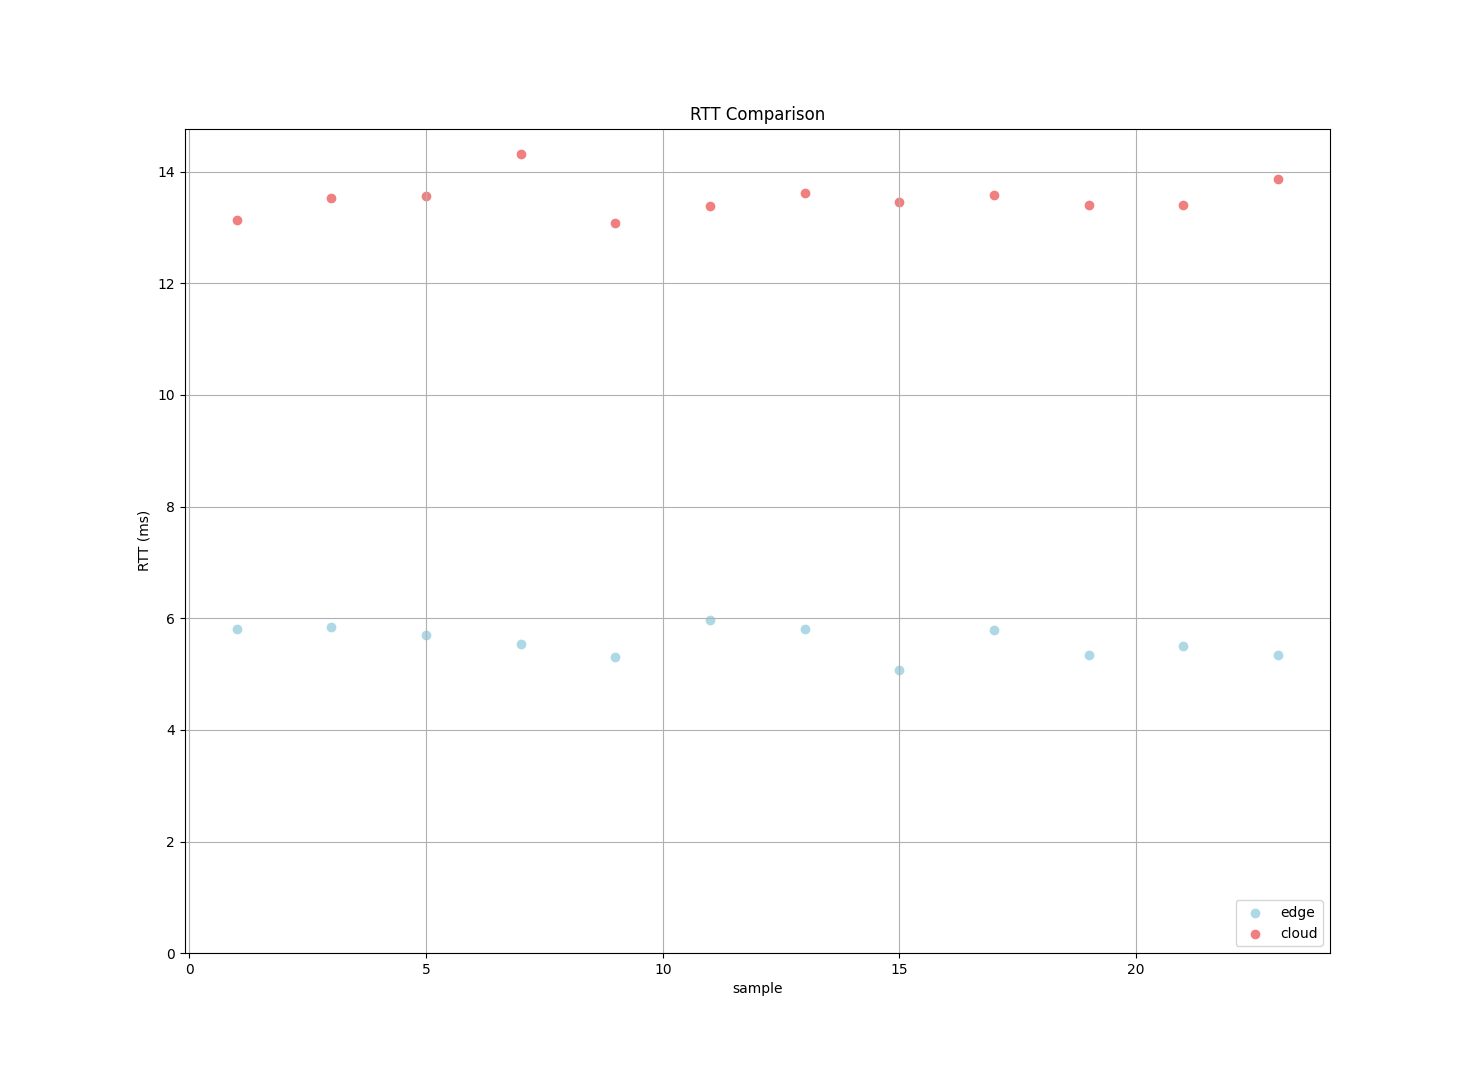
\includegraphics[width=13cm]{./images/RTT-comparison.png} 
	\caption{My PNG image}
\end{figure}
\begin{figure}[ht]
	\centering
	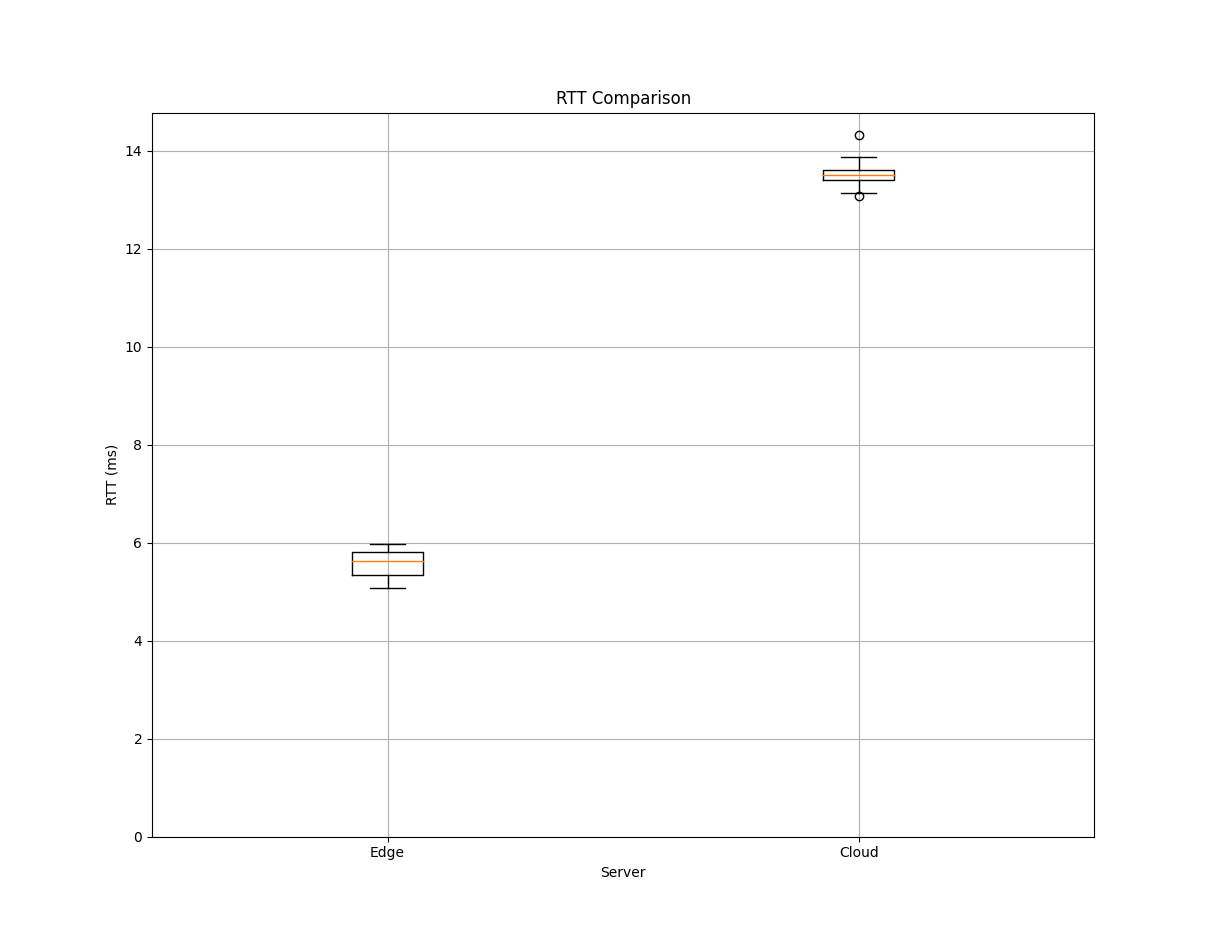
\includegraphics[width=13cm]{./images/RTT_comp_box.png} 
	\caption{My PNG image}
\end{figure}
% -----------------------
%     BIBLIOGRAPHY
% -----------------------
%\bibliographystyle{IEEEtran}
%\addcontentsline{toc}{chapter}{References}
\bibliography{thesis}


\clearpage
%\bibliographystyleNew{IEEEtran}

%
%\begin{appendices}
% \chapter{TPS project requirements}
% This project also requires the use of an equation and a graph. I decided to append that to the end of this work, since I could not think of any suitable equation or graph for the project.
% Graph \ref{only-Graph} shows a sine function with added gaussian noise. Equation \ref{Eq:Shan-H} is a Shanon Hartley theorem.

%\captionsetup[figure]{name=Graph}
%\begin{figure}[h]
%	\includegraphics[width=\textwidth]{fig1.pdf}
%	\caption{Sine function with gaussian noise}
%	\label{only-Graph}	
%\end{figure}
%
%Shanon-Hartley theorem:
%\begin{equation}
%	C = B \log_2 \left(1 + \frac{S}{N}\right)
%	\label{Eq:Shan-H}
%\end{equation}
%$C$ is the capacity in bits per second, $B$ is bandwith in Hz, $S$ and $N$ are powers of a signal and noise respectively.
%
%\end{appendices}
	
	
\end{document}